\documentclass[12pt, 
    twoside=false, 
    bibliography=totoc, 
    numbers=endperiod, 
    headings=normal, 
    toc=chapterentrydotfill
    ]{scrbook}
\usepackage[T1]{fontenc}
\usepackage[utf8]{inputenc}
\usepackage[ngerman]{babel}
\usepackage{blindtext}
\usepackage{csquotes}
\usepackage{booktabs}
\usepackage[toc]{appendix}
\usepackage{array}
\usepackage{setspace}
\usepackage{mathpazo}
\usepackage{graphicx}
\usepackage{float}
\usepackage{etoolbox}
\usepackage{pdfpages}
\usepackage{subcaption}
\usepackage{chngcntr}
\usepackage[hyphens]{url}
\usepackage[
  	pdfstartview=FitH,   
  	pdffitwindow=true,
  	colorlinks,
  	linkcolor=black,
  	anchorcolor=black,
  	citecolor=black,
  	urlcolor=black
  	]{hyperref}
\usepackage[labelfont=bf]{caption}
\usepackage[draft]{todonotes} 
\usepackage{float}
\usepackage[
    backend=biber, 
    style=authoryear-icomp, 
    eprint=false,
    url=true,
    doi=true,
    isbn=true,
    dashed=false,
    uniquename=false
    ]{biblatex}
\addbibresource{Bib.bib}

% Layoutanpassungen
\counterwithout{footnote}{chapter}
\setkomafont{sectioning}{\normalcolor\bfseries}
\renewcommand*{\chapterheadstartvskip}{\vspace*{-\topskip}}
\KOMAoptions{headsepline = true}
\setlength{\textheight}{1.05\textheight}
\AtBeginEnvironment{quote}{\singlespacing\small}
\makeatletter
% Keine Seitenvorschübe bei \Chapter
\newcommand\Chapter{%
                    \par\vspace{1.5cm}% anpassen
                    \global\@topnum\z@
                    \@afterindentfalse
                    \secdef\@chapter\@schapter}
\makeatother
\DefineBibliographyStrings{ngerman}{
   andothers = {{et\,al\adddot}},
}

\begin{document}

\begin{titlepage}
    \begin{minipage}[t]{0.6\textwidth}
    \flushleft 
    Universität Hamburg \\
    Fachbereich: Sozialwissenschaften \\
    Fachgebiet: Politikwissenschaft \\
    Seminar: Forschungsseminar Vergleichende und Regionalstudien \\ 
    Dozenten: Prof. Kai-Uwe Schnapp \\
    PD Dr. Falk Daviter \\
    Wintersemester 2018/19 \\
    \end{minipage}
    \hfill
    \begin{minipage}[t][1.7cm][b]{0.35\textwidth}
    
\includegraphics[width=\textwidth]{images/UHH-Logo_2010_Farbe_CMYK.pdf}
    \end{minipage}
    
    \vspace*{\fill}
    \begin{center}
	\vspace{1cm}\noindent {\textbf{Projektarbeit}} \vspace{0.2cm} \\
	\textbf{\Large Geschlechtsbezogene Repräsentationsunterschiede im Deutschen Bundestag \\
	\vspace {0,5cm} \small\emph{Inwiefern unterscheiden sich Redebeiträge und Verhalten von weiblichen und männlichen Abgeordneten im 19. Deutschen Bundestag bezüglich Häufigkeit, Thematik und Geschlechterneutralität}} \\
	\vspace{0.5cm}
	10.05.2019
	\end{center}
    \vspace*{\fill}
	
	\begin{minipage}[t]{0.48\textwidth}
    \flushleft 
    Gina-Gabriela Görner \\
    Matrikelnummer: 6436971 \\
    Friedensallee 15 \vspace{0.1cm} \\ 
	22765 Hamburg \vspace{0.1cm}  \\
	\href{mailto:gina-gabriela.goerner@uni-hamburg.de}{gina-gabriela.goerner@uni-hamburg.de} \\
    % Hab das geändert, e-mails schreibt man idR klein, wie webseiten. Sind nicht case-sensitiv
    \end{minipage}
    \begin{minipage}[t]{0.48\textwidth}
	\flushleft
	Josef Holnburger \\
	Matrikelnummer: 6524900 \\
	Beuthstraße 1 \vspace{0.1cm} \\
	10117 Berlin \vspace{0.1cm} \\
	\href{mailto:josef@holnburger.com}{josef@holnburger.com} \\
    \end{minipage}

\end{titlepage}


\tableofcontents
\thispagestyle{empty}

\frontmatter

\listoffigures
\addcontentsline{toc}{chapter}{\listfigurename}
\vspace*{24pt}
{\let\clearpage\relax \listoftables}	
\addcontentsline{toc}{chapter}{\listtablename}

\mainmatter

\setstretch{1.5}


\chapter{Einleitung}\label{Einleitung} 

\begin{quote}
    \enquote{Gender equality in political representation may be described within both optimistic and pessimistic stories.} \parencite[149]{celis_2018}
\end{quote}

\noindent
Die machtpolitische Gleichstellung der Geschlechter sowie die politische Ressourcenverteilung in den industrialisierten Demokratien ist in den letzten fünfzig Jahren enorm gewachsen \parencite[318]{coffe_2010}. Es gibt mehr weibliche Parlamentarierinnen (aus dem englischen \emph{Members of Parliament} = MPs) als je zuvor und eine Rekordzahl von Frauen nimmt Führungspositionen in den nationalen Regierungen \parencites{lovenduski_2005}{paxton_2007}, mit vielen wichtigen Konsequenzen für politische Ergebnisse und Prioritäten ein \parencites{bolzendahl_2007}{carroll_2001}{waring_2000}[318]{coffe_2010}. Dennoch sind derzeit weltweit weniger als ein Viertel Frauen (24,3 Prozent) in den Parlamenten vertreten \parencite{ipu_2019}. Repräsentative Institutionen werden trotz eines langen Kampfes um Gleichstellung noch immer von Männern dominiert \parencites[149]{celis_2018}[497 f.]{childs_2013}{dahlerup_2013} {bjarnegard_2013} und es ist nicht umstritten zu behaupten, dass eine Gleichstellung der Geschlechter nicht erreicht wurde \parencite[150]{celis_2018}. Eine parlamentarische Gleichstellung wird hierbei nicht nur über die Anzahl der Sitze in repräsentativen Parlamenten definiert, sondern ergibt sich durch eine Vielzahl an Faktoren. Hierzu zählen unter anderem die sprachliche Einbeziehung aller Geschlechter\footnote{In der Literatur herrscht ein Minimalkonsens darüber, dass es sich bei Geschlecht um eine soziale Konstruktion handelt \parencite[2]{meissner_2008}. Üblicherweise wird hier zwischen der sozial konstruierten Geschlechtsidentität oder Geschlechtsrolle (englisch \emph{gender}) und dem biologischen Geschlecht (englisch \emph{sex}) unterschieden \parencite[3f.]{meissner_2008}. Allerdings gibt es Menschen, welche sich keiner konstruierten binären Geschlechtisdentität zuordnen wollen oder können (oft als \emph{genderqueer}, \emph{genderfluid} oder \emph{non-binary} bezeichnet). Auch biologisch ist ein streng binäres Geschlechtermodell nicht haltbar -- intersexuelle Menschen weichen hier von einem solchen Modell ab und sind oft von Marginalisierung und Ausgrenzung betroffen \parencite[vgl.][]{richards_2016}. Um eine solche Marginalisierung zu vermeiden und auf die Vielzahl an Geschlechtern hinzuweisen, wird in dieser Arbeit eine genderinklusive Schreibweise genutzt. Die Schreibweise mittels des sogenannten \emph{Gendersternchen} (beispielsweise \enquote{Polikter*innen} soll hierbei zugleich Männer und Frauen, als auch alle weiteren Geschlechteridentitäten repräsentieren. Generell wird versucht, auf genderexklusive Begriffe (etwa \emph{Student}) zu verzichten und stattdessen eine genderinklusive Begriffe zu nutzen (\enquote{Studierende}). Da die überwiegende Forschung zur Repräsentation von Geschlechtern in Parlamente ein binäres Geschlechtermodell anwendet -- etwa der Vergleich der Anzahl der Sitze von Frauen in repräsentativen Parlamenten durch die Inter-Parliamentary Union \textcite{ipu_2019} -- wird auch in dieser Arbeit ein binäres Modell genutzt. Möglichkeiten zur besseren Repräsentation von \emph{genderqueeren} und intersexuellen Menschen in Parlamenten finden sich beispielsweise bei \textcite{squires_2008}. Eine kritische Auseinandersetzung mit der hier beschriebenen Problematik findet sich bei \parencite[6ff.]{meissner_2008}.} innerhalb der Parlamentsdebatten und das Nichtvorhandensein von geschlechtsspezifischem Verhalten sowie eine geschlechterunspezifische Themenwahl \todo[inline]{Du hattest hier noch die Grammatik angemerkt, weiß aber nicht, woran das Problem genau lag. Bitte auf die Fußnote achten, kann sein, dass das falsch gelesen wurde.!!! Immernoch nicht nachvollziehbar - in dem vorherige Satz fehlt ein Wort!!!}. Da die Gleichstellung und Repräsentation von Frauen in Parlamenten anhand der Anzahl an Sitzen im Parlament in einer Vielzahl an Erhebungen bereits untersucht wurde\footnote{Eine Vergleich der Sitzanteile von Frauen nach Ländern findet sich etwa auf der Seite der Inter-Parliamentary Union unter \url{https://www.ipu.org/resources/publications/infographics/2019-03/women-in-politics-2019}}, wird in der hier vorliegenden Arbeit eine umfassendere Untersuchung der Repräsentation von Frauen vorgenommen. 

\citereset
\begin{quote}
     \enquote{Gender equal representation is not only about the proportion of men and women legislators or the outcomes of politics}\parencite[197]{erikson_2018}
 \end{quote}

In Anlehnung an \textcite{erikson_2018} wird eine geschlechtergerechte Repräsentation in der vorliegenden Arbeit weder ausschließlich daran gemessen, ob eine gleiche Anzahl an Frauen und Männern im Parlament vertreten ist, noch anhand der politischen Ergebnisse. Ausgangspunkt dieser Arbeit für eine \emph{geschlechtergerechtere Repräsentation} ist ein mehrdimensionaler Repräsentationsbegriff:

Repräsentation gilt als ein Kernkonzept in der Erforschung und Praxis der Politik und kann in verschiedenen, miteinander vernetzten Dimensionen betrachtet werden. Es kann hierbei zwischen dem, was repräsentiert wird, wie es repräsentiert wird und wer repräsentiert, unterschieden werden \parencite[557]{galligan_2007}. In den meisten Fällen bieten sowohl die Wähler*innen, Parteien, Wahlen und Gesetzgeber*innen den Hintergrund für eine Diskussion über eine oder mehrere Elemente der jeweiligen Repräsentationsdimension \parencite[557]{galligan_2007}.
In der vorliegenden Arbeit werden fünf Repräsentations-Dimensionen definiert und differenziert voneinander betrachtet. Obwohl keine der im Folgenden genannten Dimension gänzlich unabhängig von den anderen Dimensionen analysiert werden kann, werden sie in dieser Arbeit zunächst klar voneinander getrennt um die Komplexität der verschiedenen Dimensionen zu reduzieren. Eine Hierarchisierung der Dimensionen ist kein Bestandteil dieser Analyse. Das Ziel liegt in einer differenzierten Analyse der folgenden fünf Ebenen der Repräsentation von Frauen.

\begin{itemize}
    \item Ebene A: \emph{Repräsentation von Frauen im Parlament}: Sind Frauen im Parlament vertreten? Wie viele Frauen sind relativ und absolut im Parlament vertreten? 
    \item Ebene B: \emph{Beteiligung von weiblichen MPs an den Parlamentsdebatten}: Nehmen weibliche MPs absolut und relativ (in Bezug auf die Anzahl an Sitzen im Parlament) gleich viel an den Parlamentsdebatten teil wie männliche MPs? 
    \item Ebene C: \emph{Berücksichtigung von Frauen in der Sprache der Parlamentsdebatten}: Werden in den Debatten Frauen ebenso wie Männer sprachlich repräsentiert? Wird Gender-Fair-Language (GFL) genutzt? Wird GFL von weiblichen und männlichen MPs in gleichem Maße genutzt? 
    \item Ebene D: \emph{Vermeidung von geschlechtsbezogenen Stereotypisierungen}: Werden gesellschaftliche geschlechtsbezogene Stereotypisierungen reproduziert? Werden unterschiedliche Themen von weiblichen und männlichen MPs behandelt? Gibt es thematische Unterschiede innerhalb der Reden zu den gleichen Themen zwischen männlichen und weiblichen MPs? 
    \item Ebene E: \emph{Verhinderung von frauenfeindlichen Verhaltensmustern}: Werden in den Parlamentsdebatten frauenfeindliche Verhaltensmuster reproduziert? Werden Frauen häufiger negativ unterbrochen? 
    \end{itemize}

Der anfängliche Versuch alle 5 Ebenen mit einem \emph{Repräsentationsbegriff} zu erfassen (A: Repräsentation von Frauen im Parlament, B: Repräsentation von Frauen in Parlamentsdebatten, C: Repräsentation von Frauen \emph{in} Parlamentsdebatten scheitert an den Ebenen D und E. Bei diesen beiden Ebenen geht es vielmehr um eine Reproduktion (D: die Reproduktion von Stereotypisierungen, F: die Reproduktion von frauenfeindlichen Verhaltensmustern).

Der theoretische Hintergrund, die Relevanz des Untersuchungsgegenstandes sowie bisherige Untersuchungen zur Repräsentation von Frauen sollen zunächst detailliert dargestellt werden. Auf Basis dieses Hintergrunds ist eine anschließende Entwicklung von Hypothesen sowie die Konzeption des Forschungsdesigns möglich, welche eine umfassende Untersuchung der Repräsentation von Frauen in Parlamenten ermöglicht. Hierbei wird im Besonderen auch die von \textcite[18]{back_2018} hingewiesene Möglichkeit der automatisierten Textanalyse genutzt.

Im Anschluss wird die Forschungsfrage \enquote{\emph{Inwiefern unterscheiden sich Redebeiträge und Verhalten von weiblichen und männlichen Abgeordneten im 19. Deutschen Bundestag bezüglich Häufigkeit, Thematik und Geschlechterneutralität}} umfassend untersucht. Während eine Vielzahl an Studien den Schwedischen Riksdag \parencites{!!!!!??????} \todo[inline]{würde jetzt nicht sagen, dass eine Vielzahl den schwedischen Riksdag untersuchen -- nur, dass es wenige oder keine gibt, die sowas schon beim Bundestag gemacht haben. Bäck legt halt den Fokus auf den Riksdag. Man kann ja noch als Ausnahme Bäck 2018 dazu nehmen, die einen Ländervergleich macht in dem auch Deutschland vorkommt.}fokussiert, ist der Deutsche Bundestag in Hinblick auf geschlechtsbezogene Repräsentationsunterschiede in den Parlamentsdebatten bis dato weniger bis gar nicht erforscht und daher Gegenstand dieser Untersuchung.

In der abschließenden Diskussion in Kapitel \ref{kapitel:diskussion} wird ausführlich auf die einzelnen Dimensionen der Repräsentation am Beispiel des 19. Bundestages eingegangen.\todo[inline]{hier noch einige Infos zu den Ergebnissen anschließen und die Dimensionen in die Arbeit einbauen - ...?!?!?! JH: Jap }


\Chapter{Theoretischer Hintergrund}

Nachfolgend wird die Theorie des \emph{Workplace-Approach} von \textcite{erikson_2018} und das Konzept der \enquote{\emph{culture of masculinity}} von \textcite{lovenduski_2005} sowie \textcite{erikson_2018} dargestellt, welche maßgeblich für den Hintergrund und die weitere Argumentation dieser Arbeit sind. 

\section{Workplace-Approach: Politik aus der Perspektive eines Arbeitsplatzes} 


Die bisherige Forschung zur politischen Repräsentation von Frauen fokussiert primär deskriptiven Themen, wie etwa die Frage danach, wie gesetzgebende Gremien durch Quoten geschlechtergerecht strukturiert werden können \parencites [vgl.]{dahlerup_2005}{schwindt-bayer_2009} oder substantive Themen, welche beispielsweise untersuchen, ob weibliche Gesetzgeberinnen (im Orignal: \emph{legislators}) einen positiven Einfluss auf genderfreundliche politische Ergebnisse haben \parencites [199]{erikson_2018}{beckwith_2007}. Den \emph{inneren Mechanismen} der gesetzgebenden Körperschaften sowie der Frage, \enquote{how the political game itself is gendered} wurde bisher weniger empirische Aufmerksamkeit gewidmet \parencites[199]{erikson_2018}[vgl.][]{childs_2016}{dahlerup_2013}{wangnerud_2015}.

Ein Ausgangspunkt der vorliegenden Arbeit ist, dass das legislative Arbeitsumfeld für sich genommen ebenso wichtig ist, wie die Möglichkeiten der weiblichen Gesetzgeberinnen die Ergebnisse zu beeinflussen. Politikerinnen sollten in der Lage sein, ihre Aufgaben als Gesetzgeberinnen auf Augenhöhe mit ihren männlichen Kollegen zu erfüllen \parencite[199]{erikson_2018}. 

\textcites{dahlerup_2006}{dahlerup_1988} unterscheidet zwischen zwei verschiedenen Perspektiven der substantiellen Repräsentation von Frauen. Zum einen existiert die politische \emph{Outcome-Perspektive}, welche die wissenschaftliche Literatur zur substantiellen Repräsentation von Frauen tendenziell dominiert. Zum anderen existiert die Perspektive \emph{Politik als Arbeitsplatz}, welche in der vorangegangenen Literatur weniger diskutiert wurde \parencites[513]{dahlerup_2006}[199]{erikson_2018}. 

Während sich die Outcome-Perspektive darauf konzentriert, ob weibliche Gesetzgeberinnen den Inhalt politischer Entscheidungen beeinflussen, indem sie diese geschlechtsfreundlicher gestalten oder eine feministische Agenda verfolgen, beschäftigt sich die zweite Perspektive mit den Möglichkeiten, wie weibliche MPs als Repräsentantinnen gleichberechtigt mit ihren männlichen Kollegen auftreten können \parencites[199]{erikson_2018}{dahlerup_2006}{dahlerup_1988}.

Der in dieser Arbeit verwendete \emph{\enquote{workplace approach}} oder die bereits genannte Arbeitsperspektive  (\emph{Politik aus der Perspektive eines Arbeitsplatzes}) zielt in Anlehnung an \textcite{erikson_2018} insgesamt darauf ab, die Repräsentation von Frauen aus einer breiteren Perspektive zu betrachten, indem der Fokus von den Ergebnissen auf die geschlechtsspezifischen Bedingungen innerhalb der Legislative verlagert wird. Mit Orientierung an die Arbeiten von \textcites{dahlerup_2006}{dahlerup_1988}{erikson_2018} werden die  Arbeitsbedingungen im deutschen Bundestag in der vorliegenden Arbeit als wichtig und wesentlicher Bestandteil der Möglichkeiten eingestuft, wie Frauen die politischen Ergebnisse beeinflussen können. Die sprachliche Einbeziehung von -- und das Verhalten gegenüber -- Frauen innerhalb der Parlamentsdebatten beeinflussen hierbei ebenso wie geschlechterneutrales Verhalten das Arbeitsumfeld von Poltikerinnen im Deutschen Bundestag.

Doch auch wenn sich in den niedergeschriebenen Regeln und den zugrundeliegenden Gesetzen des Bundestages keine \emph{per se} frauendiskriminierenden Passagen finden -- bis dato sind diese Insitutionen hauptsächlich durch Männer dominiert.
\todo[inline]{der letzte Satz ist etwas schwierig, ich kann noch nicht genau benennen was mich daran stört - daher kurz markiert um den nochmal im Auge zu behalten!!!!!}

\section{Legislative Gremien als maskuline Organisation}

%
Das Geschlechterregime der legislativen Gremien wird, ebenso wie andere von Männern dominierten Sektoren, häufig als \enquote{\emph{permeated by a culture of masculinity}} beschrieben \parencites[200]{erikson_2018}{lovenduski_2005}.
In Anlehnung an \textcite{acker_1990} zeigt sich dies beispielsweise in der Existenz von formalen Regeln, die von Männern geschaffen wurden und einer männlich dominierten Organisation angepasst sind, sowie in Normen, wie sich ein (männlicher) Politiker präsentieren und verhalten soll \parencites[200]{erikson_2018}[48]{acker_1990}. Frauen werden infolgedessen mit dieser bereits existenten \emph{culture of masculinity} konfrontiert, welche als institutionelle Einschränkung fungieren kann wenn beispielsweise ihre Arbeit dadurch behindert wird \parencites[200]{erikson_2018}[47-56]{lovenduski_2005}. \textcite{erikson_2018} verweisen auf sozialpsychologische Erhebungen, wonach Frauen in männerdominierten Bereichen häufiger Diskriminierung ausgesetzt sind, da es an Übereinstimmungen zwischen den männerdominierten beruflichen Normen und den Eigenschaften mit denen Frauen typischerweise assoziiert werden, mangelt \parencites[vgl.][]{burgess_1999}{eagly_2002}{heilman_2001}{heilman_2004}. 
%
Frauen riskieren Diskriminierungen, weil sie entweder als weniger kompetent angesehen werden oder weil sie weibliche Attribute verletzen, wenn sie sich den Normen anpassen \parencite[200]{erikson_2018}. Die Folgen sind neben der Disqualifikation, die Abwertung der Leistungen sowie die ungleiche Behandlung von Frauen bis hin zu Belästigungen \parencites[200]{erikson_2018}{heilman_2001}{burgess_1999}:
%

\citereset
\begin{quote}
     \endquote{The gendered consequences of masculine norms are often manifested in the first case in the disqualification of women or the devaluation of their performance, whereas they often take the form of a disparate treatment of women in the second, including harassment} \parencite[200]{erikson_2018}
\end{quote}

Informelle Praktiken und Normen innerhalb des Arbeitsumfeldes können als Hindernis für die Schaffung eines geschlechtergerechten Arbeitsumfeldes angesehen werden \parencite[200]{erikson_2018}. Ausgangspunkt der vorliegenden Arbeit ist die Annahme, dass der 19. Deutschen Bundestag ebenfalls von einer \enquote{\emph{culture of masculinity}} geprägt ist und dies neben weiteren Faktoren die Geschlechtergerechtigkeit des Arbeitsumfeldes zum Nachteil von Frauen beeinflusst.

\Chapter{Relevanz des Forschungsgegenstandes}

In demokratischen Systemen sind Parlamentarier*innen nicht nur wichtige Akteure als Gesetzgeber*innen, sondern auch als Teilnehmer*innen an der öffentlichen Debatte und als Mitwirkende an der öffentlichen Meinungsbildung \parencite[188]{dahlerup_2018}.
In Anlehnung an \textcite{back_2018} gibt es mehrere Gründe, warum die Auswirkungen des Geschlechts auf das Verhalten der legislativen Debatte interessant sind. Ein wichtiger Grund ist die zentrale Rolle der legislativen Debatte in parlamentarischen Demokratien, wonach Gesetze in der Regel von Abgeordneten diskutiert werden, bevor über sie abgestimmt wird \parencites[2]{back_2018}{back_2016}{proksch_2015}.
Die Debatten können in Anlehnung an \textcite[1]{proksch_2015} ebenso als Foren für die öffentliche Kommunikation angesehen werden, welche von den Parteien und ihren Abgeordneten für Wahlzwecke genutzt werden \parencite[2]{back_2018}. Ausgehend davon, dass die Debatten Auswirkungen auf die Politikgestaltung haben und von Parteien genutzt werden, um sowohl die Medien als auch die Wähler*innen zu informieren und zu beeinflussen, ist es von Relevanz ob Frauen unterrepräsentiert sind \parencite[2]{back_2018}. \citeauthor{back_2018} argumentieren, dass eine solche Unterrepräsentation im Gesetzgebungsprozess sowie der medialen Berichterstattung zu einem Bias gegen Frauen führen kann und das \enquote{gendered speech patterns} der Legitimität des demokratischen Systems schaden können \parencite[2]{back_2018}.
Die Relevanz von Geschlechtergleichheit auf politischer Ebene kann nicht (mehr) in Frage gestellt werden. Dennoch gibt es Uneinigkeit darüber, ob und inwiefern eine Geschlechtergleichheit bereits erreicht wurde und auf welchen Ebenen eine Gleichstellung der Geschlechter bereits abgeschlossen oder nahezu umgesetzt wurde. In Anbetracht der zunehmenden deskriptiven Repräsentation von Frauen im Parlamenten ist es essentiell, eine Analyse nicht ausschließlich auf dieser Ebene der Repräsentation durchzuführen und sich optimistisch mit einer Zunahme an Frauen in den Parlamenten zufrieden zu geben, sondern die Forderung nach Geschlechtergerechtigkeit im Sinne gleicher und gleichwertiger Repräsentation auf allen Ebenen zu fordern und fördern. 

\citereset
\begin{quote}
    \enquote{While women have made substantive progress in their representation in politics, they are still well underrepresented in political life in most nations} \parencite[2]{coffe_2013}
\end{quote}

Wenngleich ein politischer Konsens darin besteht, dass Gleichheit und Gerechtigkeit, sowie implizit Geschlechtergleichheit und Geschlechtergerechtigkeit, eine fundamentale Komponente von Demokratie darstellen, sind nach wie vor weltweit weniger Frauen (24,3\%) \parencite[]{ipu_2019} in den Parlamenten vertreten.\todo [inline]{!!!ALS FUßNOTE: Ausgenommen sind hierbei derzeit Ruanda: 61,3\%, Cuba: 53,2\% und Bolivien: 53,1\% - Stand April 2019 \parencite{ipu_2019}).}

Anne Phillips gilt als eine der wichtigsten Vertreterinnen auf dem Gebiet der parlamentarischen Repräsentativität von Frauen -- sie baut in ihrem Werk \emph{The Politics of Presence} \parencite*{phillips_1998} die Annahme auf, dass eine höhere deskriptive Repräsentation durch Sitze im Parlament auch zu einer höheren substantiellen Repräsentation von Frauen führt \parencite[52]{wangnerud_2009}. Hierfür analysiert Phillips jene Umstände, unter denen Frauen als Kandidatinnen für die Parlamentssitze ausgewählt werden, erfolgreich an Wahlen teilnehmen und Ministerinnen werden \parencite[vgl.][416f.]{blaxill_2016}. Frauen sind im täglichen Leben anderen Erfahrungen ausgesetzt als Männer. Hierbei bezieht sich \textcite{phillips_1998} unter anderem auf die Kindererziehung, Bildung, Auswahl an Berufen, Unterscheidung von bezahlter und unbezahlter Arbeit sowie auf Gewalterfahrungen und sexuellen Belästigungen. \textcite{phillips_1998} plädiert aufgrund der unterschiedlichen Lebenserfahrungen für die notwendige Repräsentation von Frauen im Parlament, um andere Frauen vertreten zu können \parencite[vgl.][52]{wangnerud_2009}.

\citereset
\begin{quote}
    \enquote{There are particular needs, interests, and concerns that arise from women's experience, and these will be inadequately addressed in a politics that is dominated by men. Equal rights to a vote have not proved strong enough to deal with this problem; there must also be equality among those elected to once} \parencite[66]{phillips_1998}
\end{quote}

Hanna F. Piktin \parencite*{pitkin_1972} argumentiert bereits 1967 in ihrem Hauptwerk \emph{The Concept of Representation}, dass der Interessenbegriff in der Repräsentationsdebatte omnipräsent (\enquote{ubiquitious}) ist \parencite[69]{wangnerud_2000}. Für Pitkin sind es die Parlamentarier\emph{innen}, welche sich den Wünschen und Interessen, dem Wohlergehen sowie den Themen der Frauen widmen und diese vertreten \parencites[vgl.][413]{blaxill_2016}{pitkin_1972}. In Anlehnung an Phillips' Theorie der \emph{politics of presence} \parencite*{phillips_1998} wird angenommen, dass weibliche Politikerinnen die Interessen und Wünsche weiblicher Bürgerinnen besser als männliche Politiker repräsentieren können. Hierbei wird die deskriptive mit der substantiellen Repräsentation verknüpft \parencite[52]{wangnerud_2009}: ein höherer Frauenanteil in Parlamenten führt zu einer stärkeren Thematisierung der Belange von Frauen.

Während die Forderungen einer deskriptiven parlamentarischen Geschlechtergleichheit ebenso wie die Forderungen nach substantieller Geschlechtergleichheit bereits ihre Wege in die wissenschaftliche Diskussion und in die Politik gefunden haben, wurde der geschlechtergerechten Sprache sowie dem geschlechtsbezogenen Verhalten in den Parlamenten bisher weniger Aufmerksamkeit gewidmet. 
Laut \textcite{menegatti_2017} ist die Sprache allerdings eine der einflussreichsten Faktoren, wodurch Sexismus und Geschlechterdiskriminierung gefördert und reproduziert werden \parencite*[1]{menegatti_2017}. \emph{Sprache} kann insbesondere die sozialen Asymmetrien von Status und Macht zugunsten des Mannes reproduzieren \parencite[1]{menegatti_2017}. Es existier[t]en einvernehmliche Normen, wonach der prototypische Mensch ein Mann ist, was sich in den Strukturen vieler Sprachen widerspiegelt und darin verankert ist. Viele grammatikalische und syntaktische Regeln sind so aufgebaut, dass weibliche Ausdrücke in der Regel von der entsprechenden männlichen Form abgeleitet werden \parencite*[1]{menegatti_2017}. Männliche Substantive und Pronomen werden hingegen häufig mit einer generischen Funktion verwendet um sich sowohl auf Männer als auch auf Frauen zu beziehen. Auf diese Weise schwinden Frauen aus der mentalen Repräsentationen \parencites{vaughan_2018}{stahlberg_2001}: Maskuline Generika lassen Leser*innen und Hörer*innen mehr in männlichen als weiblichen Personenkategorien denken \parencites[2]{sczesny_2016}{stahlberg_2007}.

Neben einer mangelnden deskriptiven Repräsentation in den meisten repräsentativen Institutionen parlamentarischer Demokratien \parencite[vgl.][]{ipu_2019} ist ebenso eine mangelnde Repräsentation von Frauen und anderen, marginalisierten Gruppen in Bezug auf viele Sprachen festzustellen. Dies kann sich doppelt negativ auf die substantielle Repräsentation von Frauen in parlamentarischen Demokratien äußern -- sie sind weder durch Sprache noch durch Anwesenheit \emph{sichtbar}. Ein solch mangelnder Einfluss auf den legislativen Prozess kann sich wiederum durch Gesetze äußern, welche sich gegen die Interessen von Frauen richten \parencite[2]{back_2018}. \todo[inline]{!!!!!letzter Satz : würde ich streichen, oder? aus welche gesetzte willst du hinaus? wieso relevant hier?} \todo[inline]{Naja, ist halt von back 2018 übernommen. Sie sagen halt: Wenn Frauen nicht beteiligt -> mgl. Gesetze, welche Frauen benachteiligen. GGNEU!!!9.5.: Ich verstehe -- dann würde ich allerdings 'in' Gesetzten äußern - anstatt 'durch' Gesetzte äußern schreiben - ok? }


\section {Derzeitiger Forschungsstand und relevante Studien}

\todo[inline]{Auch hier fände ich wieder einen einleitenden Absatz gut. Ich überlege mir gleich noch was.}

\subsection{Frauen im Parlament}

In der Forschung zu Frauen im Parlament wird generell zwischen einer deskriptiven, substantiellen und (in einigen Fällen) symbolischen Form der Repräsentation unterschieden. Bei der substantiellen Repräsentation von Frauen handelt es sich um ein bisher weniger wissenschaftlich erforschtes Feld als die Analyse der deskriptiven Repräsentation \parencite[59]{wangnerud_2009}. 
Letzteres legt den Schwerpunkt auf die Analyse der Anzahl von Frauen in repräsentativen Institutionen, ersteres untersucht hingegen die Auswirkung der Präsenz von Frauen in Parlamenten \parencites[14]{coffe_2013}[52]{wangnerud_2009}.
Die zentralen Fragen lauten hierbei:

\citereset
\begin{quote}
  \enquote{[W]hether the widely professed aspiration to feminise democracy -- and in so doing to politically empower women -- is a matter largely of symbolism or substance […]}
  \enquote{[…] wheter the priority should simply be to increase the proportion of women MPs in Parliament […] or as Hanna Pitkin argued in 1967, to represent minds as well as bodies.}
  \parencite[413]{blaxill_2016}
\end{quote}

%
Die Theorie der \emph{politics of presence} \parencite{phillips_1998} diente \textcite{wangnerud_2000} als Ausgangspunkt für ihre Forschung im Schwedischen Parlament (\emph{Testing the Politics of Presence, Women's Representation in the Swedish Riksdag}, 2000). Wägnerud prüft hierbei die Hypothese, ob weibliche Politikerinnen die Interessen von Frauen stärker vertreten als männliche Politiker und kommt zu folgendem Ergebnis: \enquote{[It is] difficult to repudiate the conclusion that women's interest are primarily represented by female politicians} \parencite[][84]{wangnerud_2000}. Laut \citeauthor{wangnerud_2000} bleibt es jedoch ausstehend welche Auswirkungen zu erwarten sind, wenn die Zahl der Frauen im Parlament steigt \parencite{wangnerud_2009}.
Die Forschung von \textcite{celis_2008} greift diese Annahme empirisch auf und untersucht, in welchem Ausmaß die Bedürfnisse und Interessen von Frauen gesteigert werden, wenn die Anzahl von Frauen in politischen Entscheidungen zunimmt \parencite[vgl. auch][4]{galligan_2016}. Ein einfacher Anstieg der Anzahl von Frauen reicht nach \textcite{celis_2008} nicht aus, um einen signifikanten Einfluss auf den Gesetzgebungsprozess zu erreichen. In Anlehnung an \textcite{caul_2001} sei es beispielsweise notwendig, dass weibliche MPs in einflussreichen, wichtigen Positionen vertreten sind, um substantielle Repräsentation zu ermöglichen \parencites{caul_2001}[vgl. auch][14]{coffe_2013}.

Die \emph{critical mass theory} von \textcite{dahlerup_1988} geht davon aus, dass die Interessen von Personengruppen (in diesem Fall Frauen) erst Wahrnehmung finden, wenn diese in einer \enquote{kritischen Masse} im legislativen Prozess beteiligt ist. Erst wenn mehr als nur ein paar wenige Frauen in einem Parlament vertreten sind, ist es ihnen möglich, effektiv zusammenzuarbeiten und \enquote{frauenfreundliche} Inhalte im legislativen Prozess zu verhindern \parencite[752]{childs_2008}.\citereset 
Die \emph{critical mass theory} wurde in zahlreichen Forschungen zur Repräsentation von Frauen thematisiert -- eine umfassende Auseinandersetzung mit der Theory und bisherigen Erkenntnissen findet sich bei \textcite{childs_2008}. 

Auch die Forschung von \textcite{back_2018} analysiert die Auswirkungen einer steigenden Anzahl an Frauen in Parlamenten und kommt zu folgendem Ergebnis: 

\citereset
\begin{quote}
  \enquote{The variation found here is, however, not in line with the hypothesis suggesting that increased descriptive representation should lead to a rise in the substantive representation so that the prediction drawn from the critical mass theory is not given support here. Instead, we find that women are more underrepresented in legislative debates when they represent parties with many female MPs.}
  \parencite[17]{back_2018}
\end{quote}


\textcite{back_2018} untersuchen hierfür länderübergreifend sieben europäische Länder bezüglich der Themen und Redeanteile weiblicher MPs und resümieren, dass Frauen in Parlamenten seltener das Wort ergreifen. Dieses Ergebnis ist nicht auf einen generell niedrigeren Anteil an Frauen in den Parlamenten zurückzuführen, so \textcite{back_2018}. Weibliche MPs in Parteien mit einem geringen Frauenanteil ergreifen sogar häufiger das Wort als weibliche MPs in Fraktionen mit einem hohen Anteil an weiblichen Mitgliedern \parencite*[17]{back_2018}. Die \emph{critical mass theory} konnte somit in der Arbeit von \textcite{back_2018} nicht nachgewiesen und sogar ein gegenteiliger Effekt beobachtet werden. Allerdings betonen die Autor*innen in ihrer Untersuchung ebenfalls, dass sich dieser Effekt bei den untersuchten Parteien und Parlamenten erheblich unterscheidet \parencite[17]{back_2018}. Eine Beleuchtung der Hintergründe eines solchen \enquote{backlash effect} -- Frauen sprechen seltener in Parlamenten bei einer größeren Präsenz von Frauen im Parlament -- und eine Kritik an der \emph{critical mass theory} findet sich zusammenfassend bei \textcite[4]{back_2018} und tiefgreifender bei \textcite{childs_2008}.

Aus den Untersuchungen von \textcite{kathlene_1994} zu US-Staatsgesetzen und \textcite{back_2014} zum schwedischen Riksdag geht hervor, dass Frauen in Debatten insgesamt seltener sprechen, während die Fallstudien von \textcite{broughton_1999}, \textcite{murray_2010} und \textcite{wang_2014} dies nicht beobachten konnten. In Anlehnung an \textcite{back_2018} kann davon ausgegangen werden, dass es eine länderübergreifende Variation der Rolle des Geschlechts in Debatten gibt \parencite[2]{back_2018}. Eine gesonderte Untersuchung der Rolle des Geschlechts in den Debatten des Deutschen Bundestags erscheint auch aus dieser Perspektive notwendig. 

In einer vorangegangenen Studie von \textcite{back_2014} konnte außerdem festgestellt werden, dass geschlechterbezogene Unterschiede bei der gewählten Themen der Reden festzustellen sind \parencite[514f.]{back_2014}. \textcite{back_2014} konnten in ihrer Untersuchung des schwedischen Parlaments nachweisen, dass Männer im schwedischen \emph{Riksdag} häufiger zu sogenanntenn \emph{hard policies} (etwa Wirtschaft, Energie, Infrastruktur) sprechen. Bei sogenannten \emph{soft policies} (Erziehung, Soiale Sicherung, Bildung) war hingegen kein Unterschied bezüglich des Redeanteils nach Geschlecht der Abgeordneten festzustellen \parencite[514f.]{back_2014}. Eine umfassende Untersuchung von Geschlechterunterschieden in Bezug auf Sprache, Thematik und Verhalten der Parlamentsmitglieder des Deutschen Bundestages ist hingegen bis zu diesem Zeitpunkt noch ausstehend, wenngleich erforderlich: 

\citereset
\begin{quote}
 \enquote{Our research clearly suggest that gender plays a role in parliamentary speech-making and the selection of the MPs who take the parliamentary floor, which calls for further comparative research on the role of gender in legislative debates in different institutional contexts and with varying degrees of descriptive representation}
  \parencite[515]{back_2014}
\end{quote}

\todo[inline]{\citeauthor{back_2014} haben in ihrer Studie nur untersucht, welcher Minister vor einer Rede spricht und danach die Thematisierung festgestellt. In der neueren, länderübergreifenden Untersuchung machen \citeauthor{back_2018} darauf aufmerksam, dass man die Thematisierung in den Reden durch neue Möglichkeiten der automatisierten Inhaltsanalyse wie beispielsweise der \emph{Latent Semnatic Analysis} bei \textcite{gustafssonsenden_2015} auf Parlamentsdebatten anwenden sollte, um diese Thematik tiefergehend zu erforschen-}

\subsection{Geschlechtsspezifische Unterschiede im Parlament}\label{kapitel:geschlechterunterschiede}

In Bezug auf die Interaktion zwischen Gesetzgeber*innen konnten frühere Untersuchungen zeigen, dass Frauen und Männer innerhalb der gesetzgebenden Gremien nicht nur unterschiedliche Politik betreiben, sondern außerdem unterschiedlich behandelt werden \parencites[201]{erikson_2018}{childs_2004}. Zudem gibt es Hinweise darauf, dass männliche MPs bei einem zunehmenden Frauenanteil im Parlament, unhöflich und respektlos gegenüber weiblichen Gesetzgeberinnen sein können \parencites[201]{erikson_2018}{kathlene_1994} und dass weibliche Gesetzgeberinnen offener Diskriminierungen und sexueller Belästigung ausgesetzt sind \parencites[201]{erikson_2018}[76]{lovenduski_2005}{lovenduski_2004}.

Die Untersuchungen von \textcite{erikson_2018} liefern neue Erkenntnisse über die Existenz von anhaltenden geschlechtsspezifischen Mustern im schwedischen Parlament. Wenngleich das schwedische Parlament im Bereich der Gleichstellung der Geschlechter formal und deskriptiv vielen anderen Ländern voraus ist, lassen die Ergebnisse dennoch auf Elemente einer \emph{maskulinen Kultur} hinweisen \parencite[211]{erikson_2018}:

\citereset
\begin{quote}
    \enquote{Although changing formal rules may end officially sanctioned gender discrimination, more than two decades of nearly genderequal descriptive representation have not been enough to change informal norms and practices and overcome all institutionalized forms of male bias} \parencite[211]{erikson_2018}
\end{quote}

 Dies ist unabhängig davon, dass es sich beim schwedischen Parlament formal um einen geschlechtergerechten Arbeitsplatz handelt und sich die Regeln und Vorschriften für weibliche und männliche MPs nicht unterscheiden \parencite[211]{erikson_2018}. In Anlehnung an \citeauthor{erikson_2018} stellt sich hierbei die Frage, aus welchem Grund weibliche MPs mehr Druck, Angst und negative Behandlungen erfahren. Es wird vermutet, dass informelle Aspekte des Arbeitsumfelds im Parlament in einer Weise geschlechtsspezifisch sind, die weibliche MPs trotz ihrer formalen und deskriptiven Geschlechtergleichstellung weiterhin benachteiligen \parencite[210]{erikson_2018}.

\citeauthor{erikson_2018} verweisen auf die Notwendigkeit einer Gleichstellungsarbeit im Parlament, welche nicht ausschließlich die formalen Aspekte der Arbeitsbedingungen berücksichtigen, sondern ebenso das Bewusstsein der MPs für die Notwendigkeit der Transformation etablierter Normen und Praktiken schärfen \parencite[211]{erikson_2018}.
Mit der vorliegenden Arbeit wird teilweise auf die Forderung von\citeauthor{erikson_2018} eingegangen, die von Ihnen festgestellten Ergebnisse mit den empirischen Studien anderer legislativen Körperschaften und unterschiedlichen formalen Bedingungen (in diesem Fall der 19. Deutsche Bundestag) zu vergleichen um jene Mechanismen zu identifizieren, welche geschlechtsspezifische Arbeitsbedingungen für die Gesetzgeber*innen fördern oder behindern \parencite[211]{erikson_2018}. Letzeres kann in dieser Arbeit allerdings nicht geleistet werden und bedarf weiterer Forschung. 

\subsection{Gender-Fair-Language zur Reduktion von Stereotypisierungen und Diskriminierung}\label{kapitel:gfl-studien}

\citereset
\begin{quote}
    \enquote{Given that language not only reflects stereotypical beliefs but also affects recipients’ cognition and behavior, the use of expressions consistent with gender stereotypes contributes to transmit and reinforce such belief system and can produce actual discrimination against women} \parencite[2]{menegatti_2017}
\end{quote}

Es konnte bereits aufgezeigt werden, dass es sich bei \emph{Sprache} um eine der einflussreichsten Faktoren handelt, wodurch Sexismus und Geschlechterdiskriminierung gefördert und reproduziert werden \parencite*[1]{menegatti_2017}. Hierbei werden insbesondere soziale Asymmetrien von Status und Macht zugunsten des Mannes reproduziert \parencite{menegatti_2017}.
Maskuline Generika werden geschlechtsspezifisch in Bezug auf männliche Personen genutzt sowie generell in Bezug auf Gruppen mit gemischten Geschlechtern und in Bezug auf Personen oder Gruppen deren Geschlecht ungewiss oder irrelevant ist, mit folgendem Ergebnis: \enquote{In this way they equate maleness and humanness} \parencite[169]{stahlberg_2007}. Durch die maskulinen Generika verschwinden Frauen aus der mentalen Repräsentationen \parencites{vaughan_2018}{stahlberg_2001}. In der feministischen Linguistik wird generell angenommen, dass maskuline Bezeichnungen weibliche Personen weniger vorstellbar und sichtbar machen \parencite[131]{stahlberg_2001}. Zudem lassen maskuline Generika die Leser*innen und Hörer*innen mehr in männlichen als weiblichen Personenkategorien denken \parencites[2]{sczesny_2016}{stahlberg_2007}. In Anlehnung an \textcite{stahlberg_2007} wird in der feministischen Sprachkritik davon ausgegangen, dass die maskulinen Generika aus einem grundlegenden Androzentrismus entspringen (\enquote{\emph{the Male-as-Norm-view}}), diesen aufrechterhalten und die Frauen unsichtbar machen \parencites[170]{stahlberg_2007}{miller_1976}{silveira_1980}.

Beispielhaft sei hier die Studie von \textcite{vervecken_2013} genannt, welche die beruflichen Interessen von belgischen und deutschen Schülerinnen und Schülern und ihre Wahrnehmung der unterschiedlichen beruflichen Erfolge von Frauen und Männern bei stereotypen Männerberufen untersuchten. Wurden bei Beschreibung der Berufe feminine und maskuline Wortpaare genutzt (z. B. Ingenieurinnen und Ingeneure oder weibliche und männliche Ingenieure), förderte dies eine ausgewogenere Wahrnehmung des Erfolgs von Männern und Frauen und stärkte das Interesse der Mädchen an sogenannten \emph{stereotypischen Männerberufen} \parencite{vervecken_2013}. Ähnliche Ergebnisse finden sich in auch in der Studie von \textcite{gaucher_2011} -- wurden in Stellenanzeigen mehr männliche als weibliche Formulierungen genutzt, fanden vor allem weibliche Studienteilnehmende diese Jobs weniger attraktiv und fühlten sich weniger angesprochen \parencite[11]{gaucher_2011}.

In Anlehnung an \textcite{sczesny_2016} können verschiedene Strategien verwendet werden, um eine sprachliche Geschlechtergerechtigkeit zu erreichen und negative Auswirkungen von männlichen Generika zu vermeiden: \emph{Neutralisierung}, \emph{Feminisierung} und die \emph{Kombination der beiden} (vgl. Abb. \ref{fig:table_sprachtypen}). Die geeignete Strategie ist hierbei abhängig von der betreffenden Sprache (grammatikalische Geschlechtssprache, natürliche Geschlechtssprache, oder geschlechtslose Sprache \parencites[vgl.][]{bussmann_2003}[][3]{sczesny_2016}. 

\begin{figure}
    \centering
    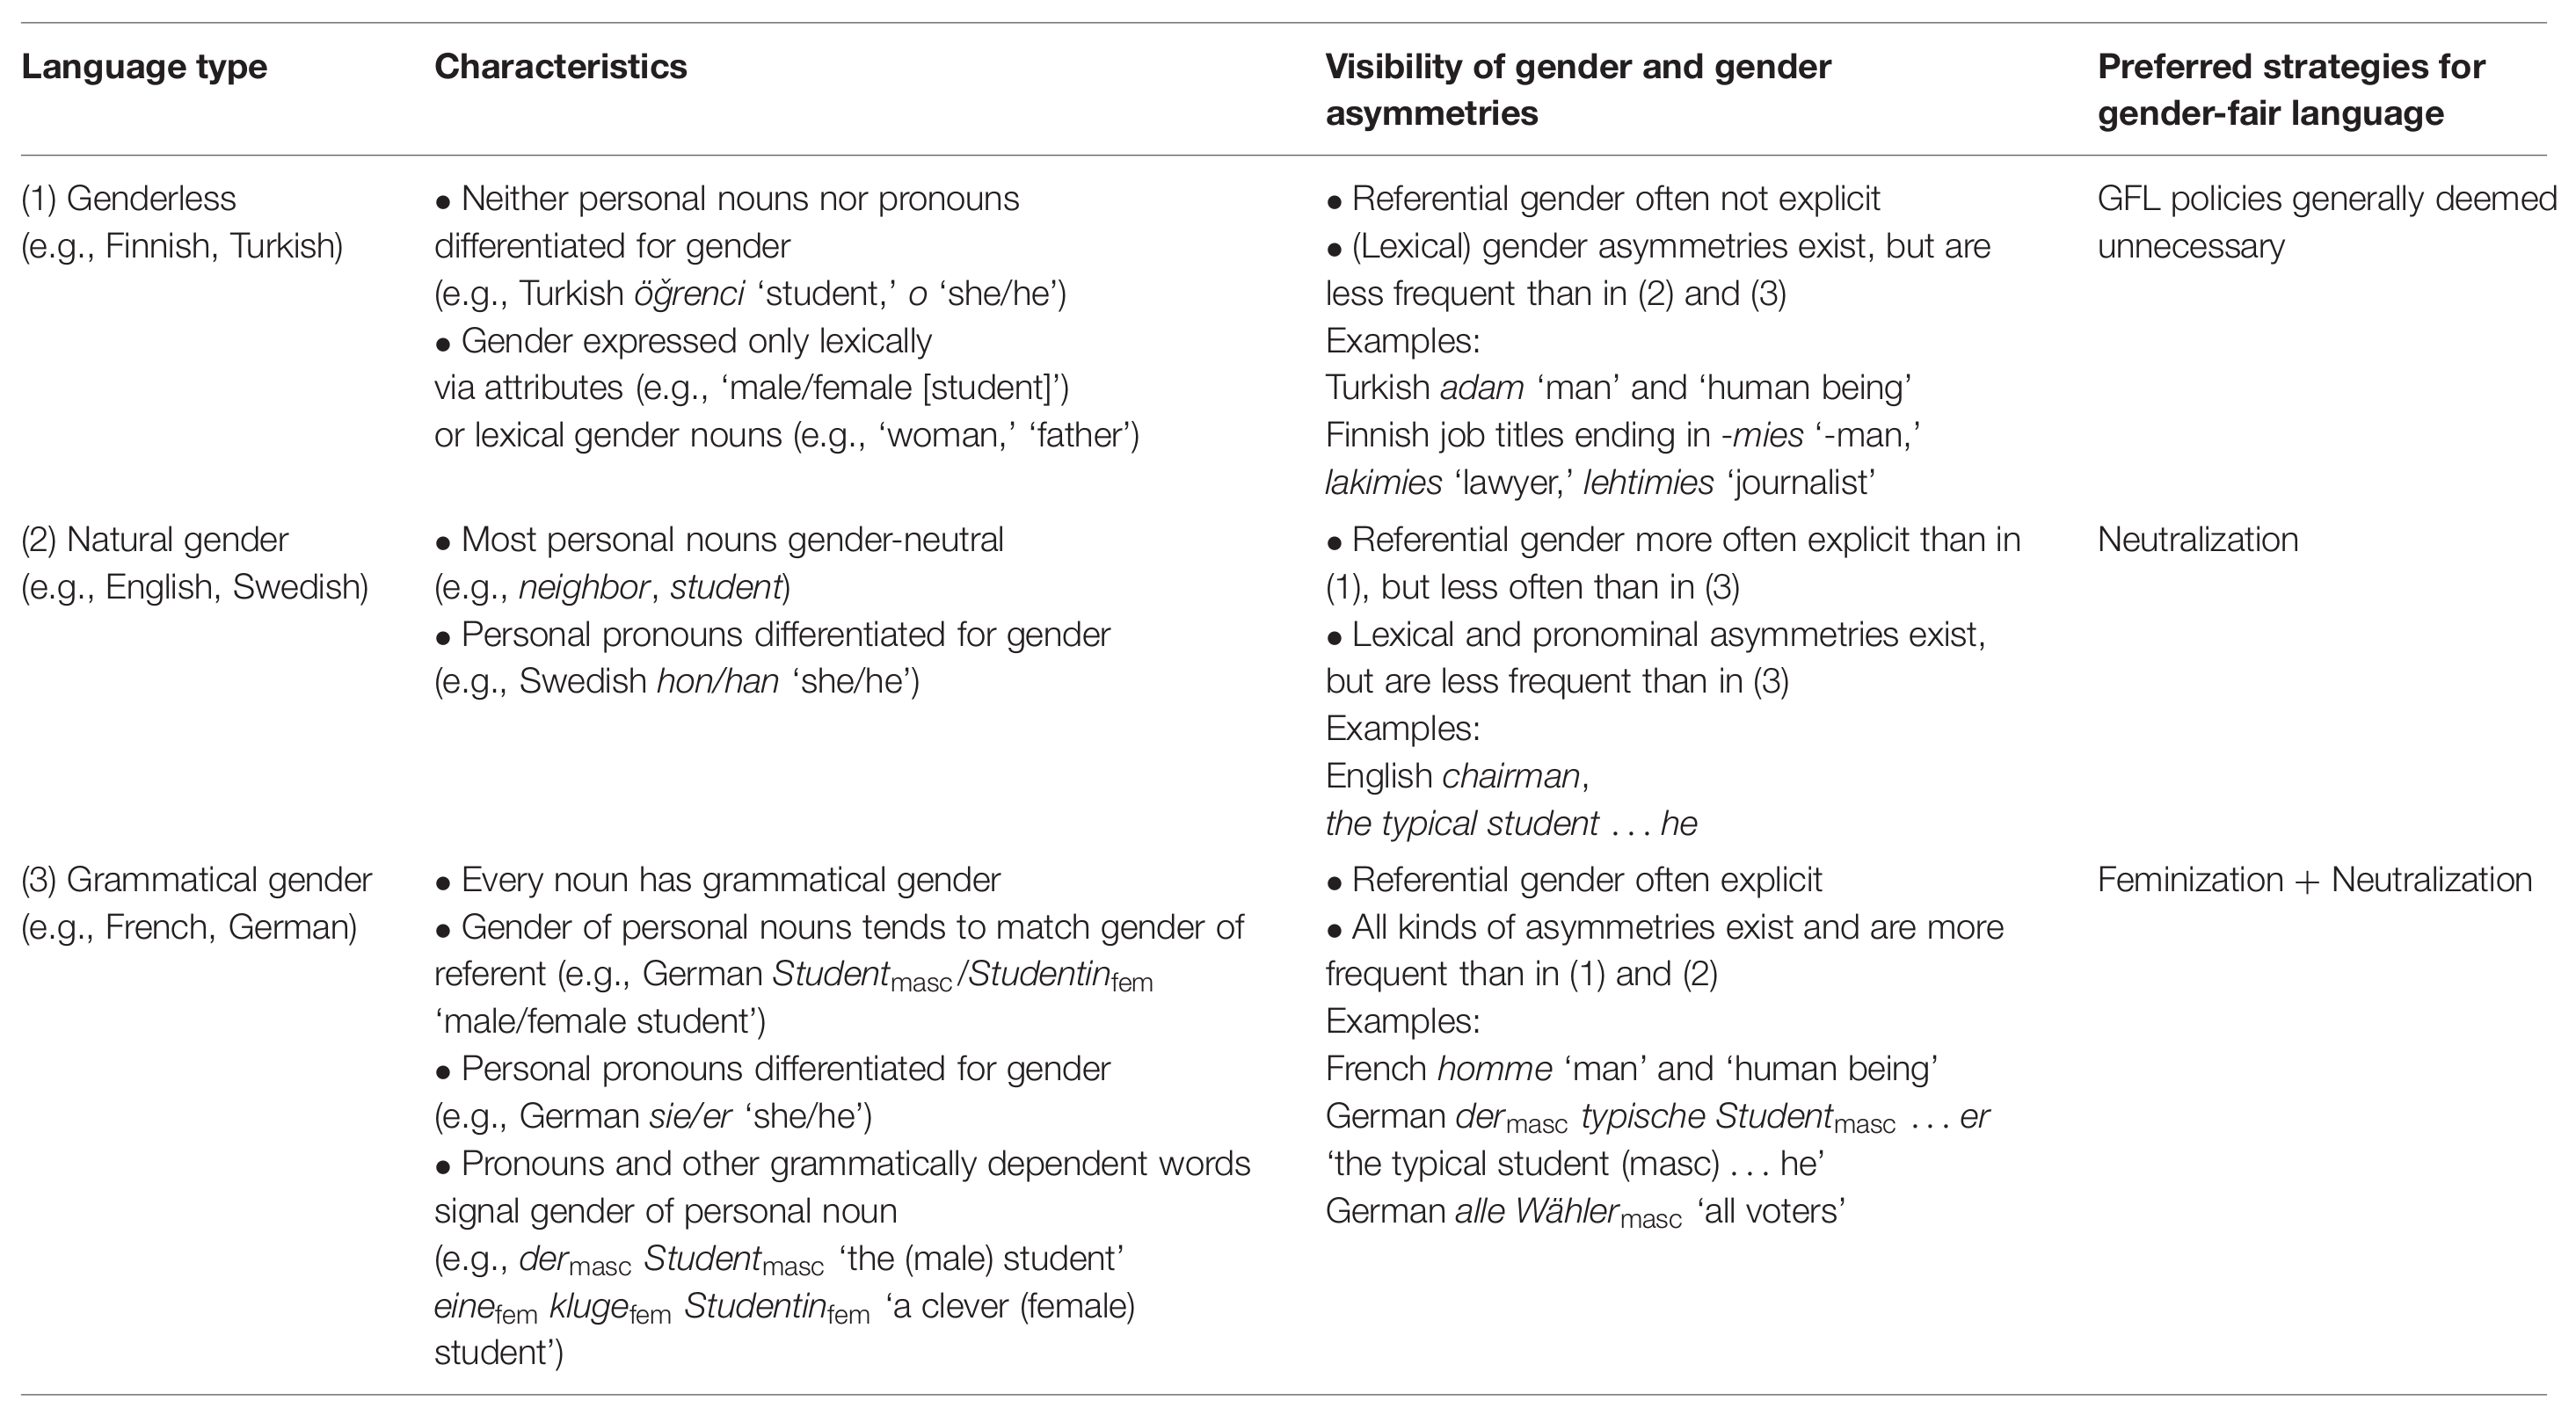
\includegraphics[width=\textwidth]{images/sczesny_table.png}
    \caption[Überblick der Sprachtypen bezüglich des Ausdrucks von Geschlecht und Geschlechtsasymmetrien]{Überblick der Sprachtypen bezüglich des Ausdrucks von Geschlecht und Geschlechtsasymmetrien. Aus \textcite{sczesny_2016} - \citetitle{sczesny_2016}}
    \label{fig:table_sprachtypen}
\end{figure}

Aufgrund der oben genannten Benachteiligungen für die Frauen ist es notwendig, die Sprachgewohnheit dahingehend zu ändern, GFL umfassend zu etablieren, um Vorurteile bezüglich der Geschlechter zu reduzieren und gleichzeitig eine Reproduktion von Stereotypisierungen zu vermeiden. Die Verwendung von geschlechtergerechten Ausdrücken anstelle von maskulinen Generika ist für den Abbau von Geschlechtervoreingenommenheit und die Förderung der Gleichstellung der Geschlechter laut Menegatti und Rubini unabdingbar \parencite*{menegatti_2017}.

Die Umsetzung und Etablierung der GFL hat in verschiedenen Ländern bisher unterschiedliche Stadien erreicht und wird beispielsweise von der UNESCO und der Europäischen Kommission empfohlen und in deren Dokumenten angewandt \parencite[4]{sczesny_2016}.

\citereset
\begin{quote}
    \enquote{[…] language does not merely reflect the way we think: it also shapes our thinking. If words and expressions that imply that women are inferior to men are constantly used, that assumption of inferiority tends to become part of our mindset; hence the need to adjust our language when our ideas evolve.} \parencite {unesco_2011}
\end{quote}

\textcite{koeser_2014} verweisen auf die Notwendigkeit einer Auseinandersetzung mit den Argumenten für die Nutzung von GFL, um den Gebrauch zu fördern:
\begin{quote}
    \enquote {The present study is the first one that investigated persuasion by arguments concerning gender-fair language. It indicates that arguments can be an effective tool for making speakers use gender-fair language.} \parencite[556]{koeser_2014}
\end{quote} 

\textcite{koeser_2014} untersuchten, inwiefern Personen ermutigt werden können, eine geschlechtergerechte Sprache zu verwenden und zu akzeptieren. Die Ergebnisse zeigen, dass Personen ihr Sprachverhalten zu einem geschlechtergerechten Gebrauch hin änderten, wenn mit entsprechenden Argumenten für die Nutzung geschlechtergerechter Sprache konfrontiert werden. Die Studie bestätigt, dass Argumente zur Förderung einer geschlechtergerechten Sprache motivieren können, geschlechtergerechte Formulierungen zu verwenden \parencite[548]{koeser_2014}. Auffällig war hierbei, dass Frauen ihren Sprachgebrauch eher in Bezug auf geschlechtergerechte Sprache ändern als Männer \parencite[555]{koeser_2014}. 


\Chapter{Übergeordete Forschungsfrage und Konzeption der Arbeit}

Während sich, wie eingangs beschrieben, eine Vielzahl der wissenschaftlichen Forschung mit der Repräsentation von Frauen in Parlamenten aus einer deskriptiven und substantiellen Perspektive auseinandersetzt, fokussiert die vorliegende Forschungsarbeit die geschlechtsspezifischen Repräsentationsunterschiede bezüglich der Parlamentsdebatten auf fünf Ebenen (siehe Kapitel \ref{Einleitung}). 

\begin{itemize}
    \item Ebene A: Repräsentation von Frauen im Parlament
    \item Ebene B: Beteiligung von weiblichen MPs an den Parlamentsdebatten
    \item Ebene C: Berücksichtigung von Frauen in der Sprache der Parlamentsdebatten
    \item Ebene D: Vermeidung von geschlechtsbezogenen Stereotypisierungen
    \item Ebene E: Verhinderung von frauenfeindlichen Verhaltensmustern
\end{itemize}

Neben dem Anteil an Reden von Frauen im Deutschen Bundestag werden die Reden des Deutschen Bundestages inhaltlich analysiert und das Verhalten der Abgeordneten in Bezug auf geschlechtsspezifische Besonderheiten untersucht. Die zentrale Forschungsfrage lautet: \enquote{\emph{Inwiefern unterscheiden sich die Redebeiträge und das Verhalten von weiblichen und männlichen Abgeordneten im 19. Deutschen Bundestag bezüglich Häufigkeit, Thematik und Geschlechterneutralität}}.


\section{Hypothese Genderinklusive Sprache}\label{kapitel:hypothese1}

Es konnte bereits aufgezeigt werden, dass die Nutzung von GFL die Benachteiligungen von Frauen systematisch senken kann. Mit Hilfe von GFL können Vorurteile bezüglich der Geschlechter reduziert und gleichzeitig eine Reproduktion von Stereotypisierungen vermieden werden. Wängnerud geht davon aus, dass weibliche Politikerinnen, in größerem Umfang als ihre männlichen Kollegen, die Interessen von Frauen vertreten \parencite[69f.]{wangnerud_2000}. Sie fasst das Interesse in drei Anliegen zusammen: Die Anerkennung von Frauen als eine soziale Kategorie; die Anerkennung des ungleichen Machtgleichgewichts zwischen den
Geschlechtern; und die Umsetzung von Regelungen, welche darauf abzielen, die Autonomie und Sichtbarkeit von Frauen in der Gesellschaft zu erhöhen und verbessern \parencite[69f.]{wangnerud_2000}. Die Ergebissen von \textcite{koeser_2014} konnten bereits aufzeigen, dass Frauen eher geschlechterinklusive Sprache verwenden. Für den 19. Deutschen Bundestag wird ebenfalls erwartet, dass sich dieses Ergebnis auch in den Reden der Abgeordneten wiederfindet (vgl. auch Kapitel \ref{kapitel:gfl-studien}).

\citereset
\begin{quote}
    \enquote {Surprisingly, women changed their language use more in the direction of gender-fair language than men.} \parencite[555]{koeser_2014}
\end{quote}


Ausgehend von diesem Ergebnis sowie den vorherigen Annahmen, stellen wir die folgende Hypothese auf: 

\textbf{Hypothese 1:} \emph{Weibliche MPs verwenden in ihren Reden häufiger GFL als männliche MPs}

Zur Untersuchung dieser Hypothese 

\todo[inline]{Hinweis darauf, dass nur genderinklusive Begriffe und Formulierungen verwendet werden, nicht genderexklusive. Vielleicht auch später bei der Methodik und Konzeption}


\section{Hypothese Themen der Reden}\label{kapitel:hypothese2}

\begin{quote}
    \enquote{Legislatures thus remain strongly gendered institutions, with a marked division of labor between men and women politicians that becomes especially visible in the realm of social policy ” \parencite[250]{ennser-jedenastik_2017}}
\end{quote}

Es gibt diverse Erklärungsansätze für eine unterschiedliche Themenwahl von männlichen und weiblichen MPs bei Parlamentsdebatten. Nach\textcite{wangnerud_1996} beispielsweise gibt es zwei mögliche Erklärungsansätze für eine \emph{horizontale Arbeitsteilung} bezüglich der Zuordnung von MPs zu den jeweiligen Gremien. Zum einen nennt \citeauthor{wangnerud_1996} hierbei die Stereotypisierungen dessen, was als \emph{männlich} oder \emph{weiblich} angesehen wird. Zum anderen kann es auch Unterschiede bezüglich der Interessen geben \parencite{wangnerud_1996}. \todo[inline]{HIER WICHTIG SPÄTER KRITISCH REAGIEREN!!!!} \todo[inline]{Hier sollten wir auch genauer zitieren, wo findet sich diese Argumentation bei Wägnerud? - GG NEU !!!: finde ich nicht. Du? } \citeauthor{back_2014} verweist diesbezüglich darauf, dass die Präferenzen und Entscheidungen der MPs nicht unabhängig von der Zugehörigkeit zu einer sozialen Gruppe und von den eigenen Lebenserfahrungen analysiert werden können. Die MPs beziehen sich bei der Entwicklung ihrer Präferenzen bewusst oder unbewusst auf ihre Biographie, so \textcite[507]{back_2014}. 
In den Jahren 1985, 1988 und 1994 wurden Umfragen der schwedischen MPs durchgeführt, anhand derer \textcite[81]{wangnerud_2000} feststellen konnte, dass es einen Zusammenhang zwischen dem Geschlecht der Politiker*innen und dem Ausmaß, in dem sie sozialpolitische Fragen verfolgen, gibt \parencites[506]{back_2014}[82]{wangnerud_2000}. Weibliche MPs sprechen in ihrem Wahlkampf vermehrt zu Themen wie Sozialpolitik, Familienpolitik, Seniorenpflege sowie dem Gesundheitswesens. Außerdem wurde von weiblichen MPs betont, dass Wohlfahrtsfragen in ihren eigenen Interessengebieten liegen. Laut \textcite[82]{wangnerud_2000} waren Politikerinnen immer die Gruppe, die sozialpolitische Themen in ihrer parlamentarischen Arbeit am stärksten verfolgt haben \parencites[vgl.][507]{back_2014}.
In ihrer Untersuchung zum schwedischen Parlament konnten \textcite{back_2014} nachweisen, dass Geschlechterunterschiede bezüglich der Themen der Reden festzustellen sind. Männer sprechen laut \textcite{back_2014} im schwedischen \emph{Riksdag} häufiger zu \emph{hard policies} (Wirtschaft, Energie, Infrastruktur). Bei \emph{soft policies} (Erziehung, Soziale Sicherung, Bildung) ist hingegen kein Unterschied bezüglich des Redeanteils und dem Geschlecht der Abgeordneten festzustellen \parencite[514f.]{back_2014}. Eine Analyse der Reden bezüglich möglicher Themenunterschiede zwischen den Geschlechtern, auf Basis der bisherigen Befunde im schwedischen Parlament (\parencites{wangnerud_2000}{wangnerud_2009}{back_2014}), ist für den 19. Deutschen Bundestag bisher noch ausstehend. Daher wird im Folgenden untersucht, ob eine geschlechtsspezifische, unterschiedliche Thematisierung in den Reden feststellbar ist: 
\todo[inline]{Teilweise haben wiir hier wieder aussagen doppelt. Ich würde sagen, mehr nach oben und in den Hypthesen eher verweisen auf die relevante Literatur.}

\textbf{Hypothese 2:} \emph{Es sind unterschiedliche Thematisierungen in den Reden der Abgeordneten feststellbar.}

Wie \textcite{back_2014} bereits aufzeigen konnte, gibt es unterschiedliche Erklärungsansätze. Eine ausführliche Auseinandersetzung mit den Ursachen der möglichen Themenunterschiede kann in der vorliegen Arbeit nicht geleistet werden. Mögliche Gründe für Themenunterschiede können (a) Entscheidungen der MPs aufgrund ihrer persönlichen Interessen, (b) Stereotype und/oder Normen in der Gesellschaft und/oder innerhalb der Parteien oder (c) Strategien, Hierarchien oder bestimmte Netzwerke innerhalb der Parteien sein \parencites[507]{back_2014}. \textcite [250]{ennser-jedenastik_2017} betont bezugnehmend auf \textcites{baekgaard_2012}{thomas_1994} dass es sich bei der Wahl von sozialpolitischen Themen seitens der weiblichen MPs um die Selbstauswahl und nicht die offene Diskriminierung dieses Musters handelt \parencite[250]{ennser-jedenastik_2017}. \textcite{herrnson_2003} berichtet, dass weibliche Kandidatinnen, die stereotypische weibliche Themen betonen und in ihren Kampangnen Frauengruppen ansprachen, durch diese Strategie einen Wahlvorteil erhielten \parencite[250]{ennser-jedenastik_2017}. Auch \textcite{celis_2018} nehmen Bezug auf die unterschiedliche Themenwahl von männlichen und weiblichen MPs und begründen diese auf potentielle Erfolgsaussichten:

\citereset
\begin{quote}
    \enquote{Women’s issues and interests can be represented with greater success when they fit the dominant views and discourses about the type of issues and interests that representatives should be concerned with. However, these have a gendered and elitist bias, and strategically framing decisions [...] to fit with these dominant conceptions, by definition, distorts the selection of the types of issues and interests that will be represented” \parencite[151]{celis_2018}}.
\end{quote}

\textcite{celis_2018} gehen in Ihrer Argumentation soweit, dass Themen und Interessen, die im Widerspruch zu einer dominanten Auffassungen stehen, strategisch und/oder unbewusst durch Themen ersetzt werden, die akzeptabler sind und eine bessere Chance auf Unterstützung haben \parencites[151]{celis_2018}{swers_2002}. 
Auf diese Weise wird die Themenwahl verzerrt und eine feministische Agenda abgeschwächt \parencite[151]{celis_2018}. Die bereits in Kapitel \ref{kapitel:geschlechterunterschiede} beschriebene \enquote{male-dominated nature of the political agenda} \parencite[151]{celis_2018} behindert die Inklusion von Frauen und fördert die Stereotypisierungen von Themen, so \textcite{celis_2018}.
Diese Förderung von Stereotypisierungen sowie eine Behinderung der Inklusion von Frauen gilt es zu vermeiden. Hierfür ist eine Analyse von möglichen Themenunterschiede zwischen den Geschlechtern in Form der \emph{Hypothese 2} essentiell. 

\section{Hypothese Unterbrechungen und Rückfragen in den Reden}\label{kapitel:hypothese3}

Eine von \textcite{erikson_2018} durchgeführte Befragung zum Arbeitsumfeld von schwedischen Abgeordneten konnte zeigen, dass weibliche MPs mehr Stress und Druck in ihrem Umfeld ausgesetzt sind und häufiger Opfer negativer Behandlungen im Parlament sind als männliche Abgeordnete. Sie werden eher in den Debatten unterbrochen, sind eher Opfer sexistischer Witze und ihre Äußerlichkeiten wird häufiger negativ kommentiert als die Erscheinung männlicher Kollegen \parencite[13]{erikson_2018}.

Diese Mehrbelastung kann laut \textcite{erikson_2018} zu höheren \enquote{Kosten} für Frauen bezüglich des parlamentarischen Engagements führen - sie müssen mit mehr negativen Erfahrungen rechnen als Männer. Entsprechend könnte dies auch ein Grund für eine geringere Beteiligung von Frauen in Parlamentsdebatten oder generell für die Partizipation von Frauen in politischen Institution darstellen \parencites[vgl.][]{erikson_2018}[vgl.][]{back_2014}.

Es wird erwartet, dass ein solches negatives Verhalten gegenüber Frauen auch im Deutschen Bundestag zu beobachten ist. Entsprechend wird untersucht, wie häufig weibliche und männliche MPs in ihren Reden \emph{negativ} unterbrochen werden. Hierfür werden Reden bezüglich der Anzahl an Zurufen, Gegenrufen, Widerspruch und Lachen über den*die Redner*in untersucht.

\textbf{Hypothese 3:} \emph{Frauen werden häufiger als Männer während einer Rede negativ unterbrochen}

\todo[inline]{ SO?? GG NEU!!!!: Eine weitere Unterbrechung der Render*innen können Rückfragen darstellen - allerdings ist hier eine eindeutige negative Intention nicht anzunehmen. Auf Basis der Arbeiten von \textcite{brescoll_2011} und \textcite{eagly_2002} wäre zu erwarten, dass weiblichen MPs bei Themen, welche stereotypisch tendenziell nicht mit Frauen verbunden werden, häufiger Inkompetenz unterstellt wird. Eine Untersuchung dieser Annahme (!!!! einfügen Fußnote: z.b. dies anhand der Anzahl an Rückfragen äußern, welche während einer Rede gestellt werden!!!!) bleibt allerdings in der vorliegenden Arbeit ausgespart}


\section{Redeanteile in Parlamentsdebatten}\label{kap:redenanteile}

Der 19. Deutsche Bundestag war bisher noch nicht Gegenstand einer Untersuchungen der unterschiedlichen Repräsentation von Frauen und Männern in Parlamentsdebatten. Im folgenden wird daher die Anzahl an Reden von weiblichen MPs (nach Fraktion) ermittelt. \textcite{back_2014} konnte zeigen, dass weibliche MPs im schwedischen Riksdag deutlich weniger Reden halten als ihre männlichen Kollegen. Inwieweit dieses Ergebnis auf den Deutschen Bundestag übertragbar ist, wird an dieser Stelle geprüft. Wieso die Anzahl an Reden relevant ist, verdeutlichen beispielsweise \textcite{back_2014}:

\citereset
\begin{quote}
     \enquote{\emph{taking a lot of time} on the floor can in some sense be compared with reaching an important post—in important debates, parties are likely to control the floor agenda} \parencites[507]{back_2014}
\end{quote}

Es kann die Behauptung aufgestellt werden, dass es für die jeweilige Partei von Bedeutung ist, welche Person wie viel Redezeit nutzt \parencite[vgl.][]{proksch_2012}. Es bleibt zu klären, wonach entschieden wird, welche Personen zu welchem Zeitpunkt wie lange reden.
%
Früheren Studien zufolge wird angenommen, dass persönliche Charaktereigenschaften der MPs einen Einfluss auf die Redezeit haben \parencite[505]{back_2014}. Eine umfassende Analyse des persönlichen Einflusses auf das legislative Verhalten wird an dieser Stelle jedoch nicht geleistet (mehr hierzu bei \textcite{saalfeld_2011}). Innerparteiliche Marginalisierungen könnten in Anlehnung an \textcite[507]{back_2014} beispielsweise einen möglichen Grund für weniger weibliche MPs in den Debatten darstellen. Als weiteren Grund wird in der Literatur die Stereotypisierung von Frauen als weniger kompetente Vertreterin angeführt oder die in Kapitel \ref{kapitel:geschlechterunterschiede} beschriebene \emph{culture of masculinity} \parencites[507]{back_2014}{lovenduski_2005}. 

Der von \textcite{back_2014} untersuchte schwedische \emph{Riksdag} unterscheidet sich allerdings hinsichtlich der parlamentarischen Gepflogenheiten vom Deutschen Bundestag und kann daher nicht direkt verglichen werden. Die Redeordnung und Redezeit wird im Bundestag über die Geschäftsordnung und den Ältestenrat festgelegt \parencite[64f.]{linn_2018}. Üblicherweise wird das Modell der \enquote{Berliner Stunde} angewandt -- die Redezeit bemisst sich hierbei über die Stärke der Fraktionen \parencite[vgl.][]{schreiner_2005}. Allerdings wurde im Ältestenrat des 19. Deutschen Bundestages hierzu noch keine Einigung gefunden \parencite[64]{linn_2018}, weshalb die Redezeit bis dato auf die in der Geschäftsordnung vorgesehenen 15 Minuten begrenzt werden. Bei längeren Reden von Sprecher*innen der Regierung verlängern sich auch die Reden der Oppositionsfraktionen. Generell können die Fraktionen eine längere Redezeit von bis zu 45 Minuten beantragen \parencite{bundestag_2019}. In der \enquote{aktuellen Stunde} des Bundestages sind die Redebeiträge der Abgeordneten auf maximal fünf Minuten begrenzt \parencites[68]{linn_2018}[]{bundestag_2019}.

Bedingt durch die Festlegung der Redezeit durch die Geschäftsordnung und den Ältestenrat sowie eine fehlende Protokollierung der Länge der Reden durch den Stenografischen Dienst des Bundestages ist ein Vergleich der Redezeiten von weiblichen und männlichen MPs weder sinnvoll, noch möglich. Im Rahmen der weiteren Untersuchung wird zur Bestimmung der Länge der Reden alternativ auf die Anzahl der Wörter in einer Rede zurückgegriffen. 
\textcite{back_2018} konnte in dem Ländervergleich keine Korrelation zwischen der Anzahl an Frauen in den Fraktionen und der Anzahl an Reden in den Parlamenten feststellen. Dennoch soll in dieser Arbeit ein Überblick über die Anzahl der Reden von Frauen im Vergleich zu den Sitzanteilen in der Fraktion aufgenommen werden -- diese Erkenntnis dient hierbei primär deskriptivem als deduktivem Erkenntnisgewinn, weshalb für diese Untersuchung keine Hypothesen gebildet werden. Die Ergebnisse dieser Untersuchung können die bisherigen Ergebnisse von \textcite{back_2018} sowohl ergänzen als auch überprüfen.

\Chapter{Datengrundlage und Methodik}\label{kapitel:datengrundlage}

Seit der 19. Wahlperiode liegen die Protokolle des Deutschen Bundestags als XML-Dateien (Extensible Markup Language) vor und die Struktur der abgelegten Protokolle sind umfassend dokumentiert \parencite{bundestag_2015}. Abgerufen werden können sie über das \emph{Open Data Portal} des Deutschen Bundestags.\footnote{\url{https://www.bundestag.de/service/opendata}} In Verbindung mit den dort abgelegten biografischen Daten aller Bundestagsabgeordneten können Aussagen über die Anzahl und den Inhalt der Reden nach Geschlecht, Alter und Fraktion getroffen werden.

Die Bundestagsprotokolle werden durch den Stenografischen Dienst des Deutschen Bundestages verfasst -- die Stenograf*innen erfassen in den Protokollen neben den Inhalten der Reden auch Zwischenrufe, Beifallsbekundungen, Lachen\footnote{Lachen kann in den Bundestagsprotokollen eher als \enquote{auslachen} oder \enquote{lachen über den Inhalt} verstanden werden - das Lachen beispielsweise über einen Witz wird in Bundestagsprotokollen als \enquote{Heiterkeit} protokolliert.} und weitere Unterbrechungen. Dies ermöglicht eine umfassende Auswertung nach Art der Unterbrechung, da sowohl eine Unterscheidung zwischen positiv intendierten Unterbrechungen (Beifall, Heiterkeit) und (zumeist) negativ intendierten Unterbrechungen (Zwischenrufe, Lachen), als auch die Anzahl an Rückfragen an den*die Redner*in feststellbar ist.

Zur Auswertung und Operationalisierung dienen unterschiedliche Methoden der quantitativen Textanalyse -- die genutzten Methoden sollen in den nachfolgenden Kapiteln kurz erläutert und das Vorgehen dargestellt werden. Die Daten werden für die quantitative Analyse mittels der Programmiersprache R \parencite{rcoreteam_2018} und der \emph{tidyverse}-Paketsammlung \parencite{wickham_2017} aufbereitet und auswertet. Des weiteren werden die Pakete \emph{xml2} \parencite{wickham_2018}, \emph{rvest} \parencite{wickham_2016}, \emph{furrr} \parencite{vaughan_2018}, \emph{stargazer} \parencite{hlavac_2018}, \emph{knitr} \parencite{xie_2014} und \emph{kableExtra} \parencite{zhu_2019} genutzt. 
Alle dieser Arbeit zugrunde liegenden Daten und die zur Auswertung und Aufbereitung entwickelten Skripte sind öffentlich zugänglich und können zur Reproduktion und Überprüfung der Ergebnisse genutzt werden.\footnote{Die Daten können über die Plattform \emph{Github} eingesehen und heruntergeladen werden: \url{https://github.com/holnburger/geschlechterunterschiede_bundestag}}

\section{Überblick der erfassten Reden}\label{kapitel:ueberblick_reden}

Bis zum 12. April 2019 wurden 8.764 Reden im 19. Deutschen Bundestag gehalten -- diese beinhalten auch Reden von Gästen und Regierungsmitgliedern. Allerdings stellt das \emph{Open Data Portal} des Bundestages umfassende (biografische) Daten (beispielsweise Geburtsjahr, Geschlecht, Wahlkreis, Ausschussmitgliedschaften) nur für Abgeordnete bereit. Da nachfolgend die Debatten im Parlament ausgewertet werden und die Reden von Regierungsmitgliedern eher einen berichtenden und die Reden von Gästen einen informellen Charakter besitzen, sollen nachfolgend nur die Redebeiträge von Abgeordneten untersucht werden.

Der Anteil an Reden von weiblichen MPs entspricht mit 31,0\% (vgl. Tabelle \ref{table:uebersicht_reden}) annähernd dem Frauenanteil im Bundestag von 31,8\% (222 Frauen)\footnote{\url{siehe-https://www.bundestag.de/abgeordnete/biografien/mdb_zahlen_19/frauen_maenner-529508}}.


\begin{table}[htb]
    \centering
    \caption{Anzahl und Anteil der Reden nach Geschlecht der Abgeordneten}
    
\begin{tabular}{lll}
\toprule
Geschlecht & Reden & Anteil\\
\midrule
männlich & 5.327 & 69.2\%\\
weiblich & 2.369 & 30.8\%\\
\bottomrule
\end{tabular}
    \label{table:uebersicht_reden}
\end{table}

Der Anteil der Sitze und die Redeanteile unterscheiden sich bei den Fraktionen teilweise erheblich (vgl. Tabelle \ref{table:vergleich_sitze_reden}). Die AfD hat mit 11,0\% den niedrigsten Frauenanteil im Parlament, der Anteil an Reden von weiblichen MPs beträgt 10,0\% und liegt damit etwas niedriger als der Anteil an Frauen in dieser Fraktion. 
Der größte Unterschied zwischen der Anzahl an Sitzen von Frauen und dem Redeanteil findet sich bei der CDU/CSU-Fraktion -- 20,7\% der Fraktion sind Frauen, allerdings halten diese nur 16,0\% der Reden. Auch die Linke und die SPD zeigen einen deutlichen Unterschied zwischen dem Anteil an Frauen in der Fraktion und den Reden von weiblichen MPs -- bei beiden Fraktionen ist der Anteil an Reden niedriger als der Anteil an Frauen. Lediglich bei den Grünen und der FDP findet sich ein höherer Redeanteil von Frauen im Vergleich zu deren Anteil an Sitzen.

Der von \textcite{back_2018} beschriebene \emph{backlash effect}, wonach ein höherer Frauenanteil in einer Fraktion zu weniger Reden von Frauen in den Parlamentsdebatten führt, kann in dieser Erhebung somit nicht bestätigt werden. Die Fraktionen unterscheiden sich diesbezüglich unsystematisch.

\begin{table}[htb]
    \centering
    \caption[Sitz- und Redeanteil von weiblichen MPs nach Fraktionen]{Sitz- und Redeanteil von weiblichen MPs nach Fraktionen. Auswertungszeitraum: 24. Oktober 2017 bis 12. April 2019}
    
\begin{tabular}{>{\raggedright\arraybackslash}p{2cm}>{\raggedleft\arraybackslash}p{2cm}>{\raggedleft\arraybackslash}p{2cm}}
\toprule
Fraktion & Sitzanteil Frauen & Redeanteil Frauen\\
\midrule
CDU/CSU & 20,7\% & 16,0\%\\
SPD & 42,8\% & 39,0\%\\
AfD & 11,0\% & 10,0\%\\
FDP & 23,7\% & 25,8\%\\
Die Linke & 53,6\% & 50,7\%\\
Bündnis 90/ Die Grünen & 58,2\% & 61,3\%\\
fraktionslos & 25,0\% & 43,9\%\\
\bottomrule
\end{tabular}
    \label{table:vergleich_sitze_reden}
\end{table}

In der weiteren Auswertung wird nicht auf die Reden von fraktionslosen Abgeordneten eingegangen. Hintergrund hierfür ist sowohl die geringe Anzahl an fraktionslosen Redner*innen im Bundestag (zum Auswertungszeitraum waren lediglich vier der 709 Abgeordneten fraktionslos\footnote{Frauke Petry und Mario Mieruch traten kurz nach der Wahl aus der AfD aus und waren von Beginn des 19. Bundestags nicht Mitglied einer Fraktion. Im November 2018 verlies der Abgeordnete Marco Bülow die SPD-Bundestagsfraktion, im Dezember 2018 trat Uwe Kamann aus der AfD-Fraktion aus.}) als auch Probleme in der Erhebung -- Marco Bülow und Uwe Kamann hielten ihre Reden sowohl als Mitglieder ihrer Fraktion (SPD bzw. AfD) und später auch als fraktionslose Abgeordnete des Bundestags. Der Redeanteil von Frauen bei fraktionslosen Abgeordneten (vgl. Tablle \ref{table:vergleich_sitze_reden}) ist deshalb stark verzerrt -- zum Teil trifft dies auch auf die Rede- und Sitzanteile bei den Fraktionen der AfD und der SPD zu, allerdings ist diese Verzerrung aufgrund einer deutlich größeren Anzahl an Reden und Sitzen vernachlässigbar.
Gleichzeitig gelten für fraktionslose Abgeordnete angepasste Regelungen bezüglich Anzahl der Reden und Redezeit im Vergleich zu den übrigen Abgeordneten \parencite[vgl.][583f.]{schreiner_2005}. Wie in Tabelle \ref{table:top_redner} ersichtlich, machen die fraktionslosen Abgeordneten Frauke Petry und Mario Mieruch besonders häufig von ihrem Rederecht Gebrauch.\footnote{Diese Tabelle berücksichtigt nur Bundestagsabgeordnete. Die meisten Reden wurden durch Angela Merkel (126), Heiko Maas (98) und Jens Spahn (76) gehalten.} Dies lässt sich unter anderem durch die insgesamt politisch schwächere Position von fraktionslosen Abgeordneten erklären \parencite[372]{morlok_2018} -- da sie kein Antragsrecht und keine Stimmrecht und Rederecht in Ausschüssen besitzen \parencite[vgl.][]{morlok_2018}, nutzen diese vor allem ihr Rederecht im Plenum.

Da sich das Redeverhalten sowie die Rechte von fraktionslosen Abgeordneten zu den Abgeordneten in Fraktionen derart unterscheidet, werden diese in der weiteren Auswertung nicht berücksichtigt, um eine Verzerrung der Ergebnisse zu vermeiden. Es werden insgesamt 8.186 Reden von insgesamt 677 Abgeordneten\footnote{Im Untersuchungszeitraum haben noch nicht alle Abgeordneten mindestens ein Mal eine Rede gehalten -- entsprechend ergibt sich die Differenz zwischen den insgesamt 709 Abgeordneten und der Anzahl an Abgeordneten in diesem Datensatz.} untersucht. 

\begin{table}[htb]
    \centering
    \caption[Abgeordnete mit den meisten Reden im 19. Deutschen Bundestag.]{Abgeordnete mit den meisten Reden im 19. Deutschen Bundestag. Auswertungszeitraum: 24. Oktober 2017 bis 12. April 2019}
    
\begin{tabular}{llr}
\toprule
Name & Fraktion & Reden\\
\midrule
Volker Ullrich & CDU/CSU & 68\\
Mario Mieruch & fraktionslos & 55\\
Frauke Petry & fraktionslos & 50\\
Alexander Graf Lambsdorff & FDP & 48\\
Katja Keul & Bündnis 90/ Die Grünen & 38\\
Johann Saathoff & SPD & 37\\
Sebastian Brehm & CDU/CSU & 37\\
Jürgen Hardt & CDU/CSU & 36\\
Helge Lindh & SPD & 36\\
Fabio De Masi & Die Linke & 36\\
\bottomrule
\end{tabular}
    \label{table:top_redner}
\end{table}

\section{Quantitative Textanalyse}

Die stetig zunehmende Rechenleistung, die ständige Weiterentwicklung von Methoden der quantitativen Textanalyse sowie die immer größer werdenden, zu analysierenden Datenmengen\footnote{Ein besonders prägnantes Beispiel ist hier der \emph{Manifesto Corpus}. Mit diesem Projekt wurden 1.800 maschinenlesbare Dokumente politischer Parteien aus 40 verschiedenen Ländern zur quantitativen Textanalyse veröffentlicht \parencite{merz_2016}.} haben in den vergangenen Jahren zu einem stetig steigenden Interesse der Politikwissenschaft an der Auswertung von Text als Daten (\enquote{\emph{text-as-data}}) geführt \parencite[vgl.][]{wilkerson_2017}\footnote{Eine Zusammenfassung der zahlreichen Methoden der automatisierten, quantitativen Texterfassung und eine Beleuchtung der Möglichkeiten und auch Fallstricke dieser Methoden findet sich bei \textcite{grimmer_2013}}. 
Auch in dieser Arbeit werden diese weiterentwickelten Methoden genutzt, um die für diese Forschung benötigte Datenmenge erfassbar und auswertbar zu machen.

Hierbei soll unter anderem auf die Möglichkeiten einer diktionärbasierten Inhaltsanalyse sowie einer automatisierten Erfassung von Themen (das sogenannte \emph{automated topic modeling}) zurückgegriffen werden -- beide Methoden der quantitativen Textanalyse werden in den nachfolgenden Kapiteln vorgestellt und anhand des Untersuchungsgegenstandes sowie dessen Operationalisierung genauer erläutert.


\subsection{Diktionärbasierte Inhaltsanalyse}\label{kapitel:diktionär}

Mittels sogenannter Diktionäre\footnote{In der überwiegend englischsprachigen Literatur wird von \emph{ditionaries} gesprochen. In Ermangelung eines besseren Begriffes, wird in der vorliegenden Arbeit der Begriff \enquote{Diktionär} gewählt, alternativ könnte hier auch von Wörterbüchern gesprochen werden.} können Texte einfach klassifiziert werden \parencites[274]{grimmer_2013}[166]{brosius_2012}. In Diktionären können Wörter oder Phrasen beispielsweise mit Themen oder Stimmungen verknüpft werden -- über einfaches Zählen von Wörtern in einem Dokument können anschließend Aussagen über dieses vorgenommen werden.
So kann etwa überprüft werden, ob in Zeitungsberichten oder Parteiveröffentlichungen ein Thema eher negativ oder positiv besetzt ist und daraus Rückschlüsse über die öffentliche Berichterstattung und Rezeption der Parteien gezogen werden \parencites[vgl.][]{haselmayer_2017}[vgl.][]{backfried_2016}. Allerdings ist hierbei zu beachten, dass eine diktionärbasierte Textanalyse sehr stark kontextabhängig ist -- ein Diktionär sollte immer einen Bezug auf die zu untersuchende Domäne aufweisen und außerhalb dieser Domäne nicht genutzt werden \parencite[268]{grimmer_2013}. Ein Diktionär, welches zur Bestimmung der Tonalität von Reden im Parlamenten ausgearbeitet wurde (beispielsweise das Diktionär von \textcite{haselmayer_2017}) kann nicht einfach auf auf die Analyse von Beiträgen auf den Sozialen Netzwerken herangezogen werden -- die Syntax, Semenatik und das Vokabular unterscheidet sich hier deutlich zwischen den Domänen \parencite[vgl.][534f.]{wilkerson_2017}.

Im Rahmen dieser Arbeit soll ein diktionärbasierter Ansatz zur Untersuchung der Nutzung von genderinklusiver Sprache (Hypothese 1 -- siehe Kapitel \ref{kapitel:hypothese1}) herangezogen werden. Ein solcher Einsatz eignet sich ideal, um diese Hypothese zu überprüfen. Mittels eines Wörterbuchs bestehend aus genderinklusiven und genderexklusiven Wörtern und Phrasen kann hierbei untersucht werden, ob weibliche MPs in Bundestagsreden häufiger auf genderinklusive Wörter und Formulierungen zurückgreifen als männliche MPs.  

Allerdings konnte in der umfassenden Recherche im Vorfeld dieser Arbeit kein wissenschaftlich erarbeitetes Wörterbuch gefunden werden, welches genderinklusive und genderexklusive Begrifflichkeiten und Formulierungen enthält. Idealerweise wird ein solches Wörterbuch entweder interdisziplinär erarbeitet. Das \emph{SentiWS}-Wörterbuch von \textcite{remus_sentiws_2010} wurde beispielsweise mit Beteiligung von Informatiker*innen und Linguist*innen entwickelt. 
Ein anderer Ansatz ist die Erarbeitung durch eine Vielzahl an Beteiligten, welche unabhängig voneinander Bewertungen beispielsweise zu negativer oder positiver Konotation von Wörtern und Sätzen abgeben -- ein solches Vorgehen wurde über \emph{crowdcoding} beispielsweise bei \textcite{haselmayer_2017} realisiert.

Beide Ansätze können im Rahmen dieser Arbeit nicht realisiert werden, da die entsprechenden Ressourcen nicht zur Verfügung stehen. Um dennoch ein geeignetes Diktionär zu entwickeln, wurde an dieser Stelle auf andere Möglichkeiten zurückgegriffen:
Ein ehrenamtlich gepflegtes \emph{Genderwörterbuch} auf der von Johanna Usinger und Philipp Müller betriebenen Webseite \url{www.geschicktgendern.de} pflegt durch Unterstützung von Freiwilligen \enquote{gendergerechte Alternativen} zu \enquote{üblchen Begriffen} ein und erweitert sich ständig. Im Rahmen dieser Arbeit wurde dieses Online-Wörterbuch mittels sogenanntem \emph{web scraping} \parencite{wickham_2016} abgegriffen und anschließend manuell als Diktionär aufbereitet. 

Hierbei mussten zahlreiche Einträge entfernt werden, da sie für die zu untersuchende Domäne zu spezifisch (etwa die genderexklusive Formulierung \enquote{… Um an unserer Klinik als Arzt arbeiten zu können, müssen Sie die Approbation im Original vorlegen.}) oder zu unspezifisch (\enquote{Eltern} als genderinklusive Variante von \enquote{Mütter}) erschienen. Einige genderexklusive Wörter wurden noch ohne genderinklusive Variante aufgeführt (\enquote{noch kein passender Begriff gefunden; senden Sie Ihren Vorschlag über das Kontaktformular}) -- auch diese wurden aus der Erhebung entfernt. Ein Auszug des Diktionärs über genderinklusive und -exklusive Wörter findet sich in Tabelle \ref{table:beispiele_woerter}. Der Tabellenauszug zeigt ebenfalls, dass einige genderinklusive Alternativen zu den jeweiligen Begriffen durchaus problematisch sein können -- die Gleichsetzung von \enquote{Schüler} und \enquote{Kinder} ist nicht immer möglich und manchmal auch falsch. Entsprechend muss dies bei der weiteren Auswertung und der Kritik berücksichtigt werden.


\begin{table}[htb]
    \centering
    \caption[Auszug an genderexklusiven und -inklusiven Begriffen nach Aufbereitung der Daten]{Auszug an genderexklusiven und -inklusiven Begriffen nach Aufbereitung der Daten}
    
\begin{tabular}{ll}
\toprule
Genderexklusive Begriffe & Genderinklusive Varianten\\
\midrule
Unternehmer & selbstständige Person\\
Verbraucher & Konsumierende\\
Familienhelfer & Familienhilfe\\
Sozialversicherungsfachangestellter & in der Sozialversicherung fachangestellte Person\\
Mutterschutz & Elternschutz\\
Lehrling & lernende Person\\
Protagonist & Schlüsselfigur\\
Befürworter & Unterstützung\\
Organisatoren & Organisationsteam\\
Polizisten & Polizei\\
\bottomrule
\end{tabular}
    \label{table:beispiele_woerter}
\end{table}

Die in Kapitel \ref{kapitel:gfl-studien} und \ref{kapitel:hypothese1} behandelte \emph{gender-fair language} umfasst jedoch mehr als nur einzelne Begriffe. In dieser Arbeit soll auch herausgefunden werden, ob Abgeordnete in ihren Reden eine genderinklusive Ansprache wählen -- beispielsweise, ob von \enquote{Kolleginnen und Kollegen} anstatt exklusiv von \enquote{Kollegen} oder \enquote{Kolleginnen} gesprochen wird\footnote{Der Stenografische Dienst des Bundestages protokolliert leider nicht, ob Abgeordnete mit einem sogenannten \emph{Gender-Gap} sprechen -- also bewusste Pausen vor der geschlechtsspezifischen Endung genutzt werden, etwa bei \emph{Kolleg\_innen} \parencite[vgl.][]{reisigl_2017}. Gender-Gaps werden in den Bundestagsprotokollen als rein weibliche Aussprache protokolliert.}. 


Mittels sogenannter \emph{regular expressions} \parencite{thompson_1968} können die Protokolle nach solchen genderinklusiven Formulierungen untersucht werden -- hierfür wird mit Hilfe von spezifisch definierten Regeln nach diesen Passagen im Datensatz gesucht. In dieser Arbeit wurde nach Passagen gesucht, welche alle folgende Regeln erfüllen:
\begin{itemize}
    \setlength\itemsep{0em}
    \item Zwei Wörter, welche durch ein \enquote{und} oder \enquote{oder} getrennt werden.
    \item Eines dieser Wörter endet mit den Buchstaben \enquote{in} oder \enquote{innen}, das zweite Wort endet hingegen mit \enquote{e}, \enquote{er} oder \enquote{en}.
    \item Die Wörter bestehen aus jeweils mindestens vier Buchstaben vor den jeweiligen Endungen.
\end{itemize}

Mit diesen Regeln konnten zunächst 507 Formulierungen identifiziert werden, welche nach einer manueller Bereinigung auf 417 genderinklusive Formulierungen gekürzt wurden\footnote{Hierbei wurden zum einen Formulierungen, die durch diese Regelungen nicht gefunden werden können, etwa \enquote{Männer und Frauen}, manuell ergänzt und Formulierungen, welche nicht inklusiv sind aber diesen Regeln entsprechen, entfernt. So fand sich beispielsweise auch vier Mal die Kombination \enquote{Hitler und Stalin} -- welche die formulierten Regeln erfüllt.}. Ein Auszug der aufbereiteten Daten findet sich in sich in Tabelle \ref{table:rnd_gender_phrasen}. 

%

\begin{table}[htb]
    \centering
    \caption[Auszug genderinklusiver Ansprachen nach Aufbereitung der Daten]{Auszug genderinklusiver Ansprachen nach Aufbereitung der Daten. 
    Die Kleinschreibung ist technisch bedingt.}
    
\begin{tabular}{l}
\toprule
Formulierung\\
\midrule
verkehrsteilnehmerinnen und verkehrsteilnehmer\\
rechtsanwältinnen und rechtsanwälte\\
grüninnen und grünen\\
betrügerinnen und betrüger\\
beamtinnen und beamten\\
spenderin oder spender\\
sparerinnen und sparer\\
mütter oder väter\\
zivilistinnen und zivilisten\\
trägerinnen und träger\\
\bottomrule
\end{tabular}
    \label{table:rnd_gender_phrasen}
\end{table}

%

Auf diese Weise wurde für diese Arbeit ein Diktionär entwickelt, welches genderexklusive Begriffe und genderinklusive Varianten sowie Formulierungen enthält. Kritisch ist hierbei die bereits beschriebene Datengrundlage zu bewerten -- da diese nicht wissenschaftlich entwickelt sondern durch einem ehrenamtliches Projekt entstammen, sind die Ergebnisse und Rückschlüsse der Arbeit, welche auf diesem Diktionär basieren, entsprechend mit Vorsicht zu betrachten.
Für zukünftige weitere Erhebungen benötigt es ein möglichst interdisziplinäre entwickeltes Diktionär, welches für die Untersuchung deutschsprachiger (politischer) Texte und Reden geeignet ist. Eine Grundlage oder Inspiration hierfür könnte das im Rahmen dieser Arbeit entwickelte Diktionär mit insgesamt 427 genderinklusiven Formulierungen, 1.059 genderinklusiven und 605 genderexklusiven Begriffen sein (vgl. Tabelle \ref{table:zusammenfassung_dict}.

\begin{table}[htb]
    \centering
    \caption[Zusammenfassung der Daten des entwickelten Diktionärs]{Zusammenfassung der Daten des entwickelten Diktionärs}
    
\begin{tabular}{rr}
\toprule
Übliche Begriffe & Genderinklusive Begriffe\\
\midrule
699 & 1242\\
\bottomrule
\end{tabular}
    \label{table:zusammenfassung_dict}
\end{table}

Mittels des Diktionärs kann nun der Anteil genderinklusiver Begriffe und Formulierungen in den jeweiligen Reden untersucht und Hypothese 1 (siehe Kapitel \ref{kapitel:hypothese1}) überprüft werden. Es ist allerdings zu berücksichtigen, dass ein bloßes zählen geschlechterinklusiver Begriffe und Formulierungen nicht ausreichend für die Hypothesenprüfung ist:
Die unterschiedliche Länge der Reden bedingt, dass längere Reden vermutlich mehr geschlechterinklusive Passagen enthalten. Sehr kurze Reden\footnote{Beispielsweise sei hier die Wahl des Bundestagspräsidenten bei der ersten Sitzung des 19. Bundestages genannt: \enquote{Der Kollege Dr. Wolfgang Schäuble ist vorgeschlagen. -- Ich darf Sie fragen: Sind Sie bereit, zu kandidieren?} Dr. Wolfgang Schäuble (CDU/CSU): \enquote{Ja, Herr Präsident.}. Die Antwort Wolfgang Schäubles wird als Rede in den digitalen Protokollen des Bundestages vermerkt.} enthalten hingegegen vermutlich keine genderinklusiven Begriffe und Formulierungen. Aufgrund dieser Umstände wird der Anteil an geschlechterinklusiven Wörtern im Verhältnis zur Länge der Reden untersucht. 
Reden, welche kürzer als 100 Wörter sind (460 von den untersuchten 81.86 Reden) werden in der Analyse nicht berücksichtigt, da diese sich im Charakter von der übrigen Plenardebatte deutlich unterscheiden. Hierbei handelt es sich zumeist um Antworten an das Präsidium oder Rückfragen an Redner*innen.

Mittels einer Boxplot-Grafik können die Mittelwerte und die Streuung der Anteile genderinklusiver Begriffe sowie die Formulierungen in den Reden anschließend visualisiert werden. Ein t-Test \parencite[vgl.][164ff.]{diaz-bone_2018} ermöglicht anschließend eine Hypothesenprüfung gegen die Nullhypothese $H_0$ (\emph{Frauen und Männer verwenden in ihren Reden GFL gleich häufig.}).

\subsection{Automatisierte Erfassung von Themen der Reden} \label{kapitel:methode_inhalte}

\citeauthor{back_2018} weisen in ihrer ländervergleichenden Untersuchung bereits auf die Möglichkeiten der automatisierten Erfassung von Themen und Stimmung in Texten (\enquote{automated
content analysis methods}) hin \parencite*[18]{back_2018}. Mittels solcher automatisierter Inhaltsanalysen ist es möglich, große Datensätze auszuwerten und zu erfassen. Zwar ist es auch mit qualitativen Methoden zunhemend möglich, große Textmengen zu bearbeiten und zu bewerten \parencite[vgl.][]{raediker_2019} -- allerdings sind trotz computergestützter und immer komplexerer Auswertungssoftware auch dem Grenzen gesetzt. Ein Großteil der Codierung muss weiterhin manuell erfolgen und Kategorien müssen eigenständig definiert werden \parencite[52f.]{raediker_2019}. 

Bei der automatisierten Inhaltsanalyse ist ein manueller Eingriff nicht nötigt -- hier wird einem Rechner die Aufgabe des Codierens übertragen \parencite[161]{brosius_2012}. Ziel ist es meist, die behandelten Themen in einem Dokument automatisiert zu erfassen \parencite[36f.]{niekler_2018} und zu analysieren. \emph{Topic modeling} ermöglicht es, durch Algorithmen und statische Methoden große Datenmengen nach Themen zu durchsuchen und damit zum einen Themen zu entdecken oder aber die Datenmengen überhaupt besser erfassbar und organisierbar zu machen \parencites[vgl.][77ff.]{blei_2012}[vgl.][163]{brosius_2012}\footnote{Die Begriffe \emph{Thema} und \emph{Topic} werden im weiteren Verlauf der Arbeit synonym verwendet.}. Das simpelste automatisierte \emph{topic model} ist dabei die \emph{Latent Dirichlet Allocation} (LDA) \parencite[78]{blei_2012}. Generell wird davon ausgegangen, dass ein Dokument mehrere Themen aufweist \parencites[78]{blei_2012}[88]{niekler_2018} und dass ein gemeinsames Thema sich durch ein gemeinsames, begrenztes Vokabular auszeichnet.
Ein solches gemeinsames Vokabular eines Themas ist in Abbildung \ref{fig:lda_example} schematisch dargestellt.

\begin{figure}
    \centering
    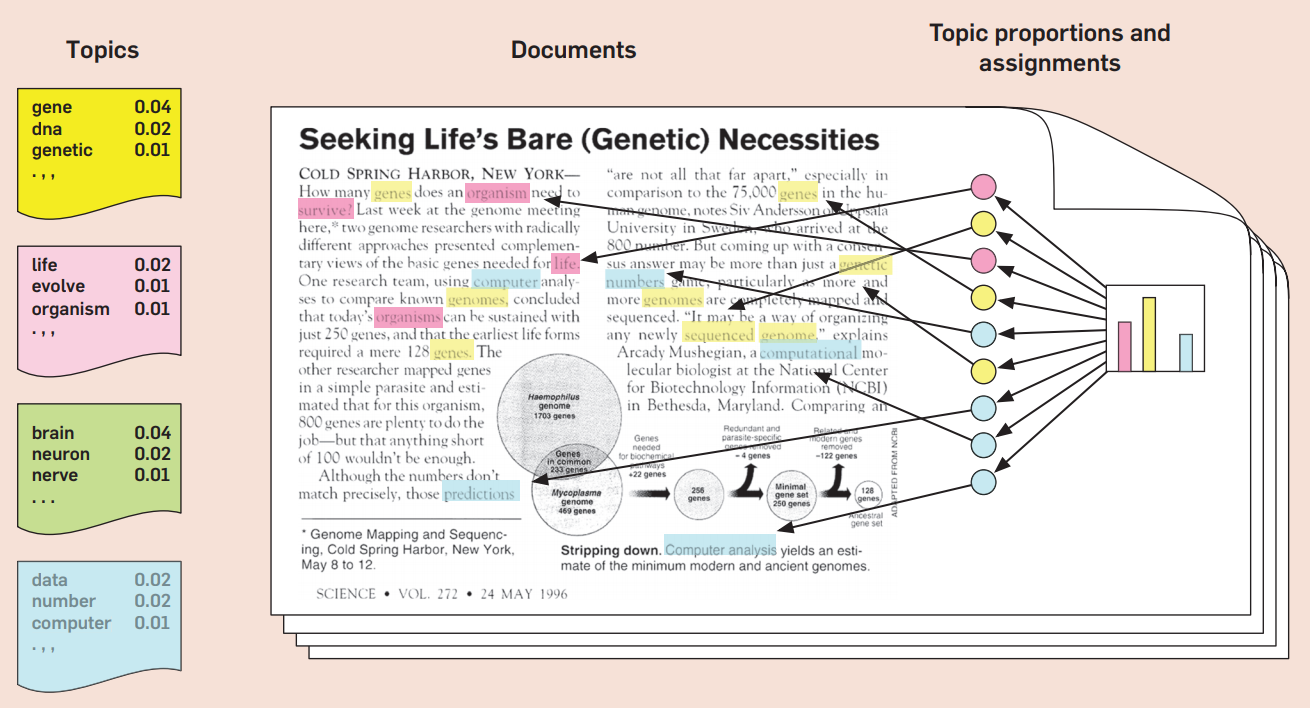
\includegraphics[width=0.8\textwidth]{document/images/lda_topic_model.png}
    % Der Teil in eckigen Klammern ist der Kurztitel für das Table of Contents
    \caption[Schematische Darstellung eines LDA Topic Models]{Schematische Darstellung eines LDA Topic Models. Quelle: \citetitle{blei_2012} \parencite{blei_2012}}
    \label{fig:lda_example}
\end{figure}

Das gemeinsame Auftreten von Wörtern in einem Dokument weist darauf hin, dass diese Wortmengen untereinander in einer Beziehung stehen \parencite[90]{niekler_2018}. Dieses gemeinsame Auftreten von Wortpaaren und Wortmengen kann untersucht werden und diese Wörter wiederum automatisiert einem Topic zugeordnet werden. Das Schema in Abbildung \ref{fig:lda_example} zeigt, wie eine solche Zuordnung aussehen kann: Die blau markierten Wörter können hierbei beispielsweise dem Thema \emph{data analysis}, gelbe markierte Wörter dem Thema \emph{genetics} zugeordnet werden \parencite[vgl.][78]{blei_2012}. Über diese Zuordnung können auch Rückschlüsse über die Häufigkeit von Themen in einem Dokument gezogen werden -- in diesem Fall behandelt das Dokument vermutlich vorwiegend das Thema \emph{genetics} (siehe \emph{Topic proportions and assignments} in Abbildung \ref{fig:lda_example}).\footnote{Bei LDA handelt es sich um ein probabilistisches Model, d. h. dass Wörter mit einer bestimmten Wahrscheinlichtkeit einem Topic zugeordnet werden können. Die technischen Details von LDA werden genauer bei \textcite{blei_2012} und die Hintergründe weiterer Topic Models bei \textcite[87ff.]{niekler_2018} beschrieben.} Trotz einer automatisierten Erfassung der Wörter eines Topics muss die Bewertung und Benennung eines Topics weiterhin manuell erfolgen und Bedarf einer Auseinandersetzung mit dem Text sowie dem Inhalt der Dokumente -- demnach kann nicht die ganze Arbeit an den Rechner abgeben werden.

Während es sich bei LDA um eines der am häufigsten gewählten und simpelsten Topic Model-Ansätze handelt, ist es für die Analyse der Themen im Bundestag ist es aus mehreren Gründen nicht geeignet:
Eine Analyse mittels LDA setzt z.B. voraus, dass die Anzahl der Themen eines Datensatzes bekannt und fix ist \parencites[93]{niekler_2018}[82f.]{blei_2012}. Auch eine Verknüpfung der Topics mit Medatdaten des Dokuments (Autor, Datum, oder -- für diese Analyse besonders relevant -- das Geschlecht des*der Autor*in) ist mit LDA nicht möglich \parencites[94]{niekler_2018}[82f.]{blei_2012}. 

Aus diesen Gründen wird auf das kürzlich entwickelte \emph{structural topic model} (STM) zurückgegriffen -- eine Variante von LDA, welche die beschriebende Limitierung durch Erweiterungen umgehen kann \parencite[640]{mishler_2015}.\footnote{STM wurde 2018 mit dem \emph{Statistical Software Award} der {Society of Political Methodology} (SPM) ausgezeichnet und für zuletzt für eine Vielzahl an Pubikationen genutzt. Die Breite der Anwendungsmöglichkeiten zeigt sich schon durch die Vielfältigkeit der Untersuchungsgegenstände: Etwa die Untersuchung von Twitter-Nachrichten während der Ukraine Krise \parencite{mishler_2015}, eine Analyse der Texte Francis Bacons des 17. Jahrhunderts \parencite{grajzl_2019} oder die -- dieser Untersuchung sehr nahen -- Studie über die Reden des 18. Deutschen Bundestages zur sogenannten \emph{Flüchtlingskrise} \parencite{geese_2019}.}

Mittels der Protokolle des 19. Deutschen Bundestages und STM ist es möglich, sowohl die Häufigkeit als auch den Inhalt der Themen der Parlamentsdebatten zu bestimmen und Unterschiede in den Thematisierungen nach Geschlecht der Abgeordneten festzustellen. Anders als \textcite{back_2014} kann somit \emph{ohne Vorannahmen} bezüglich der Themenwahl von männlichen und weiblichen MPs vorgegangen werden und eine vorherige Unterteilung in \emph{soft} und \emph{hard policies}, welche geschlechtsspezifisch favorisiert würden, kann ausgespart bleiben. Mittels dieser Methode ist es außerdem möglich, Themen zu entdecken, welche bisher noch nicht als vermeintlich geschlechtsspezifisch identifiziert wurden.

Um die Hypothese 2 (siehe Kapitel \ref{kapitel:hypothese2}) zur Thematisierung von Reden nach Geschlecht zu untersuchen, werden zunächst die Anzahl der Themen sowie die mit diesen Themen verbundenen Wörter bestimmt. Anschließend werden die Topics mit einem oder mehreren Schlagwörtern (\emph{Label}) versehen. Um diese Labels möglichst präzise zu definieren, werden sowohl die zehn Wörter, welche mit der höchsten Wahrscheinlichkeit (\emph{highest probablity}) in diesem Topic vorkommen und die Wörter, welche am exklusivsten\footnote{Hierfür wird der \emph{FREX}-Algorithmus, welcher auf der Arbeit von \textcite{airoldi_2016} basieren \parencite[12]{roberts_2018}, genutzt. Dieser wichtet die in den Topics vorhandenen Wörter nach ihrer Gesamthäufigkeit und wie exklusiv diese in diesem Topic im Vergleich zu den anderen Topics vorkommen \parencite[13f.]{roberts_2018}.} in diesem Topic vertreten sind, individuell ausgewertet und verglichen \parencite[13f.]{roberts_2018}. 

Es ist davon auszugehen, dass auch Topics gefunden werden, welche nicht mit einem Label versehen werden können -- etwa ein Topic, welches nur aus Begrüßungs- und Verabschiedungsfloskeln besteht\footnote{Da diese Wortkombinationen besonders gehäuft auftreten, wird hier ein gemeinsames Topic vermutet -- allerdings ist es für diese Auswertung nicht interessant, da jeder Redebeitrag im Bundestag mit einer Begrüßung beginnt.}. Auch Topics, welche sich nicht sinnvoll zusammenführen lassen, sind bei automatisierten Topic Models üblich \parencites[262]{mimno_2011}[11]{grajzl_2018}. Diese Topics werden, wenn beide Autor*innen übereinstimmen, aus der weiteren Auswertung entfernt. Bei Uneinigkeit bezüglich der Labels der Topics werden die Reden, welche vor allem dieses Topic beinhalten, herangezogen und anschließend ein Label vergeben.

Abschließend dann eine Untersuchung bezüglich der Thematisierung nach Geschlecht der Abgeordneten möglich -- hierbei wird untersucht, ob ein signifikanter Unterschied zwischen den beiden Gruppen (männliche und weibliche Abgeordnete) zu beobachten ist \parencite[vgl.][3]{roberts_2013}. 


\subsection{Erfassung von Unterbrechungen}

Da der Stenografische Dienst des Bundestages nicht nur den Wortlaut der Reden sondern auch Unterbrechungen, Zustimmung, Rückfragen und auch sonstige Zwischenfälle dokumentiert, es es möglich, die Unterbrechungen der Reden auszuwerten (vgl. Abb. \ref{fig:protokoll_bsp}). Hierbei kann zwischen positiv intendierten Unterbrechungen (Beifall, Heiterkeit, Zustimmung) und negativ intendierten Unterbrechungen (Widerspruch, Zwischenruf, Lachen\footnote{Der Stenografische Dienst dokumentiert das Lachen beispielsweise über einen Witz als Heiterkeit im Unterschied zu (aus)lachen.}) unterschieden werden.
Sofern möglich, dokumentieren die Stenograf*innen des Bundestags auch, wer den Zwischenruf geäußert hat und wie der Zwischenruf lautete. Diese Dokumentation ist auch in den XML-Dateien der Bundestagsprotokolle (siehe Kapitel \ref{kapitel:datengrundlage}) vorhanden und kann genutzt werden, um die Anzahl der Unterbrechungen pro Rede auszuwerten.

Wie in Kapitel \ref{kap:redenanteile} bereits erläutert gibt es bezüglich der Redezeiten im 19. Deutschen Bundestag nicht die bis dato übliche Regelung der sogenannten Berliner Stunde \parencite[vgl.][]{schreiner_2005}. Die Redezeit der Abgeordneten darf somit nicht länger als 15 Minuten sein, wobei längere Reden beantragt werden können und bei längeren Berichten der Bundesregierung auch der Opposition ein längeres Rederecht zugestanden wird. Es ist davon auszugehen, dass längere Beiträge häufiger unterbrochen werden. Deshalb wird für die weitere Auswertung nicht die absolute Anzahl an Unterbrechung sondern die Unterbrechungen im Verhältnis zur Länge der Rede in Wörtern untersucht.

Des Weiteren wird davon ausgegangen, dass Fraktionsvorsitzende und stellvertretende Fraktionsvorsitzende ebenfalls häufiger unterbrochen werden, da sie eher bei Themen sprechen, welche eine größere Medienaufmerksamkeit bedienen und hierbei oft mehr Abgeordnete anwesend sind\footnote{Eine besonders intensive Auseinandersetzung mit Unterbrechungen und deren Häufigkeiten findet sich in der Auswertung \enquote{Das gespaltene Parlament} der Süddeutschen Zeitung von 24. April 2018 \parencite{sueddeutsche_2018}}.

Aus diesen Gründen soll, neben der Rolle des Geschlechts bei Unterbrechungen, auch untersucht werden, ob (stellvertretende) Fraktionsvorsitzende im Vergleich zu anderen Abgeordneten häufiger unterbrochen werden und ob sich Unterschiede bei den Parteien bezüglich negativ intendierter Unterbrechungen feststellen lassen.

Mittels einer Boxplot-Grafik können die Mittelwerte und die Streuung der Unterbrechungen in den Reden visualisiert werden. Ein t-Test \parencite[vgl.][164ff.]{diaz-bone_2018} ermöglicht anschließend eine Hypothesenprüfung gegen die Nullhypothese $H_0$ (\emph{Frauen und Männer werden in den Reden gleich häufig negativ unterbrochen.}). Es wird anschließend verglichen, ob ein Unterschied bei Fraktionsvorsitzenden bezüglich der Unterbrechungen festzustellen ist. Unterschiede zwischen den Parteien werden über eine Varianzanalyse überprüft.

\Chapter{Ergebnisse und Auswertungen}

\section{Genderinklusive Sprache}

Wie umfänglich dargelegt, wird vermutet, dass weibliche MPs häufiger als ihre männlichen Kollegen Gebrauch von genderinklusiven Begriffen und Formulierungen machen (siehe Kapitel \ref{kapitel:gfl-studien} und \ref{kapitel:hypothese2}). Eine Überprüfung mittels dieses für diese Arbeit eigens entwickelten Diktionärs (vgl. Kapitel \ref{kapitel:diktionär}) zeigt jedoch, dass keine signifikanten Unterschiede in der Nutzung von genderinklusiver Sprache zwischen den Geschlechtern festzustellen ist. Zwar zeigt das Ergebnis des t-Test (\textit{t}(4324.78)~=~-8.84, \textit{p}~<~.001, \textit{d}~=~-0.22), dass die Nullhypothse $H_0$ (\emph{Frauen und Männer verwenden in ihren Reden gender-fair language gleich häufig.} zugunsten der Alternativhypothese $H_1$ (\emph{Frauen verwenden in ihren Reden häufiger gender-fair language als Männer} abgelehnt werden kann -- allerdings sind die Unterschiede in der Nutzung von GFL marginal (vgl. Abb. \ref{fig:boxplot_gfl}). 

\begin{figure}[H]
    \centering
    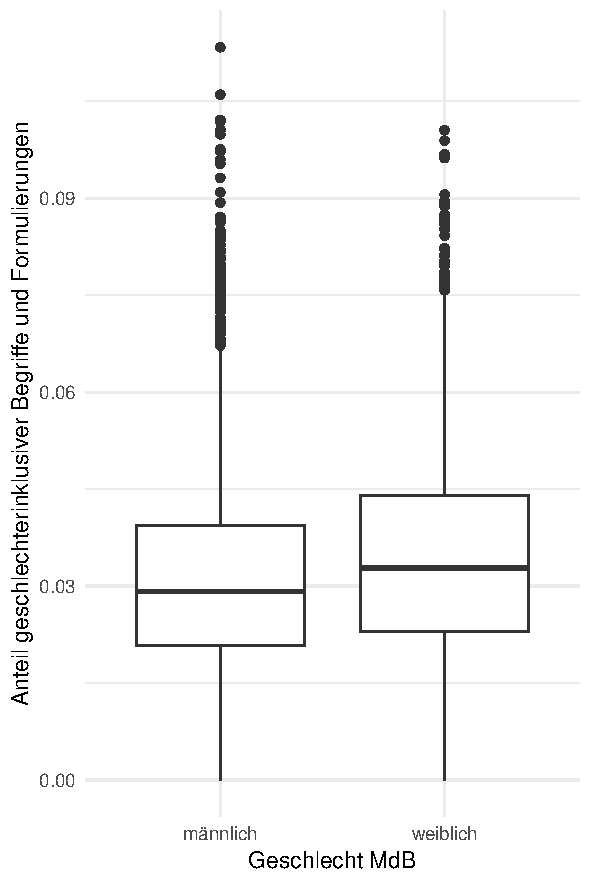
\includegraphics[width=0.7\textwidth]{document/images/boxplot_gfl.pdf}
    \caption[Anteil geschlechterinklusiver Begriffe und Formulierung pro Rede im Deutschen Bundestag]{Anteil geschlechterinklusiver Begriffe und Formulierung pro Rede im Deutschen Bundestag.}
    \label{fig:boxplot_gfl}
\end{figure}


\todo[inline]{Kritik an dem entwickelten DIktionär bzgl. der geschickt gendern -> teilweise findet zu viel (einbauen der 10 häufigsten und 10 wenigsten) genderinklusoven Wörter -> kritik DOmänenabhängigkeit : geschickt-gendern hier ein unpassendes Wörterbuch für die Untersuchung politischer Reden. Auch eine Betrachtung der GFL ohne Formulierungen wie "Kolleginnen und Kollegen" zeigen hier keine Unterschiede. Diktionär ist deshalb ungenügend für die Auswertung. Sie auch: Häufigster inklusiver Begriff \enquote{alle} -- dieser findet sich im geschickt-gendern Wörterbuch als genderinklusive Variante von \enquote{jeder}. Er sit allerdings so unspezifisch, dass er die Erhebung verzerrt. Im Vergleich zu den anderen Begriffen wird er 22.231 mal in den Reden gefunden, der zweithäufigste inklusive Begriff \enquote{frei} findet sich 7.095 mal in den Reden -- dieser wird auf der geschickt-gendern Webseite als genderinklusive Variante von \enquote{herrenlos} vorgeschlagen, wird in den Reden allerdings vermutlich eher unspezifischer verwendet. Auch Parteien werden untersucht.}


\begin{table}[htb]
    \centering
    \caption[Die zehn häufigsten genderinklusiven Formulierungen in den Reden des Bundestages]{Die zehn häufigsten genderinklusiven Formulierungen in den Reden des Bundestages. Die Kleinschreibung ist technisch bedingt.}
    
\begin{tabular}{ll}
\toprule
Genderinklusive Formulierungen & n\\
\midrule
damen und herren & 9.480\\
kolleginnen und kollegen & 7.668\\
bürgerinnen und bürger & 1.055\\
soldatinnen und soldaten & 639\\
mitarbeiterinnen und mitarbeiter & 245\\
arbeitnehmerinnen und arbeitnehmer & 244\\
verbraucherinnen und verbraucher & 199\\
mieterinnen und mieter & 179\\
ärztinnen und ärzte & 165\\
schülerinnen und schüler & 124\\
frauen und männer & 115\\
patientinnen und patienten & 95\\
kollegen und kolleginnen & 83\\
zuhörerinnen und zuhörer & 81\\
sozialdemokratinnen und sozialdemokraten & 80\\
steuerzahlerinnen und steuerzahler & 79\\
beamtinnen und beamten & 72\\
männer und frauen & 70\\
rentnerinnen und rentner & 69\\
erzieherinnen und erzieher & 68\\
wählerinnen und wähler & 62\\
polizistinnen und polizisten & 58\\
migrantinnen und migranten & 45\\
zuschauerinnen und zuschauer & 39\\
mann und frau & 37\\
politikerinnen und politiker & 37\\
helferinnen und helfer & 35\\
mütter und väter & 35\\
lehrerinnen und lehrer & 33\\
vertreterinnen und vertreter & 33\\
athletinnen und athleten & 32\\
wissenschaftlerinnen und wissenschaftler & 30\\
beamtinnen und beamte & 29\\
expertinnen und experten & 29\\
journalistinnen und journalisten & 29\\
mitbürgerinnen und mitbürger & 29\\
unternehmerinnen und unternehmer & 29\\
nutzerinnen und nutzer & 26\\
europäerinnen und europäer & 25\\
genossinnen und genossen & 25\\
arbeitgeberinnen und arbeitgeber & 24\\
demokratinnen und demokraten & 24\\
landwirtinnen und landwirte & 23\\
besucherinnen und besucher & 22\\
rednerinnen und redner & 22\\
richterinnen und richter & 22\\
freundinnen und freunde & 21\\
künstlerinnen und künstler & 19\\
pflegerinnen und pfleger & 19\\
väter und mütter & 19\\
parlamentarierinnen und parlamentarier & 17\\
kurdinnen und kurden & 16\\
ministerinnen und minister & 14\\
vorrednerinnen und vorredner & 14\\
einwohnerinnen und einwohner & 13\\
forscherinnen und forscher & 13\\
beitragszahlerinnen und beitragszahler & 12\\
kundinnen und kunden & 12\\
autofahrerinnen und autofahrer & 11\\
diplomatinnen und diplomaten & 10\\
seniorinnen und senioren & 10\\
teilnehmerinnen und teilnehmer & 10\\
betreuerinnen und betreuer & 9\\
bürger und bürgerinnen & 9\\
soldaten und soldatinnen & 9\\
staatsbürgerinnen und staatsbürger & 9\\
vater und mutter & 9\\
akademikerinnen und akademiker & 8\\
gründerinnen und gründer & 8\\
herren und damen & 8\\
urheberinnen und urheber & 8\\
zöllnerinnen und zöllner & 8\\
bewerberinnen und bewerber & 7\\
bewohnerinnen und bewohner & 7\\
brüder und schwestern & 7\\
kandidatinnen und kandidaten & 7\\
pendlerinnen und pendler & 7\\
polizeibeamtinnen und polizeibeamten & 7\\
sauenhalterinnen und sauenhaltern & 7\\
spätaussiedlerinnen und spätaussiedler & 7\\
sportlerinnen und sportler & 7\\
vermieterinnen und vermieter & 7\\
berichterstatterinnen und berichterstatter & 6\\
christinnen und christen & 6\\
haushälterinnen und haushälter & 6\\
kameradinnen und kameraden & 6\\
mieter und mieterinnen & 6\\
partnerinnen und partner & 6\\
sparerinnen und sparer & 6\\
spitzenforscherinnen und spitzenforscher & 6\\
studentinnen und studenten & 6\\
therapeutinnen und therapeuten & 6\\
unterstützerinnen und unterstützer & 6\\
vorgängerinnen und vorgänger & 6\\
afghaninnen und afghanen & 5\\
aktivistinnen und aktivisten & 5\\
anwältinnen und anwälte & 5\\
arbeitnehmer und arbeitnehmerinnen & 5\\
britinnen und briten & 5\\
bundesbürgerinnen und bundesbürger & 5\\
bundespolizistinnen und bundespolizisten & 5\\
dieselfahrerinnen und dieselfahrer & 5\\
jesidinnen und jesiden & 5\\
käuferinnen und käufer & 5\\
mütter oder väter & 5\\
mutter und vater & 5\\
petentinnen und petenten & 5\\
staatssekretärinnen und staatssekretäre & 5\\
trainerinnen und trainer & 5\\
anlegerinnen und anleger & 4\\
anwohnerinnen und anwohner & 4\\
arbeiterinnen und arbeiter & 4\\
ärzte und ärztinnen & 4\\
asylbewerberinnen und asylbewerber & 4\\
betriebsrätinnen und betriebsräte & 4\\
bezieherinnen und bezieher & 4\\
freifunkerinnen und freifunker & 4\\
fußgängerinnen und fußgänger & 4\\
grüninnen und grüne & 4\\
mama und papa & 4\\
mitarbeiter und mitarbeiterinnen & 4\\
mitberichterstatterinnen und mitberichterstatter & 4\\
musliminnen und muslime & 4\\
nachwuchswissenschaftlerinnen und nachwuchswissenschaftler & 4\\
praktikerinnen und praktiker & 4\\
russinnen und russen & 4\\
schäferinnen und schäfer & 4\\
türkinnen und türken & 4\\
volksvertreterinnen und volksvertreter & 4\\
zivilistinnen und zivilisten & 4\\
amtsträgerinnen und amtsträger & 3\\
arbeitgeber und arbeitgeberinnen & 3\\
aufbauhelferinnen und aufbauhelfer & 3\\
ausbilderinnen und ausbilder & 3\\
ausländerinnen und ausländer & 3\\
aussiedlerinnen und aussiedler & 3\\
autorinnen und autoren & 3\\
berlinerinnen und berliner & 3\\
botschafterinnen und botschafter & 3\\
empfängerinnen und empfänger & 3\\
fahrradfahrerinnen und fahrradfahrer & 3\\
handwerkerinnen und handwerker & 3\\
journalisten und journalistinnen & 3\\
kämpferinnen und kämpfer & 3\\
konsumentinnen und konsumenten & 3\\
kritikerinnen und kritiker & 3\\
kunden und kundinnen & 3\\
mann oder frau & 3\\
minijobberinnen und minijobber & 3\\
nutzer und nutzerinnen & 3\\
organspenderin oder organspender & 3\\
pädagoginnen und pädagogen & 3\\
patienten und patientinnen & 3\\
professorinnen und professoren & 3\\
raucherinnen und raucher & 3\\
reservistinnen und reservisten & 3\\
schriftstellerinnen und schriftsteller & 3\\
schulabgängerinnen und schulabgänger & 3\\
spenderinnen und spender & 3\\
staatsanwältinnen und staatsanwälten & 3\\
unternehmer und unternehmerinnen & 3\\
vater oder mutter & 3\\
wissenschaftler und wissenschaftlerinnen & 3\\
absolventinnen und absolventen & 2\\
akteurinnen und akteure & 2\\
ansprechpartnerinnen und ansprechpartner & 2\\
antragstellerinnen und antragsteller & 2\\
arbeitnehmerinnen und arbeitgeber & 2\\
ärztinnen oder ärzte & 2\\
bundesministerinnen und bundesminister & 2\\
fachpolitikerinnen und fachpolitiker & 2\\
fahrerinnen und fahrer & 2\\
feministinnen und feministen & 2\\
geschäftsführerinnen und geschäftsführer & 2\\
heldinnen und helden & 2\\
juristinnen und juristen & 2\\
klägerinnen und kläger & 2\\
kommunalpolitikerinnen und kommunalpolitiker & 2\\
landwirte und landwirtinnen & 2\\
medizinerinnen und mediziner & 2\\
minister und ministerinnen & 2\\
mutter oder vater & 2\\
nachfolger und nachfolgerinnen & 2\\
pilotinnen und piloten & 2\\
präsidentinnen und präsidenten & 2\\
radfahrerinnen und radfahrer & 2\\
rechtsanwältinnen und rechtsanwälte & 2\\
retterinnen und retter & 2\\
schüler und schülerinnen & 2\\
sozialdemokraten und sozialdemokratinnen & 2\\
tunesierinnen und tunesier & 2\\
urheberrinnen und urheber & 2\\
venezolanerinnen und venezolaner & 2\\
verfasserinnen und verfasser & 2\\
vertreter und vertreterinnen & 2\\
verwaltungsrichter und verwaltungsrichterinnen & 2\\
vorredner und vorrednerinnen & 2\\
wanderarbeiterinnen und wanderarbeiter & 2\\
alevitinnen und aleviten & 1\\
altenpflegerinnen und erzieherinnen & 1\\
anhängerinnen und anhänger & 1\\
anlagenbetreiberinnen und anlagenbetreiber & 1\\
antifaschistinnen und antifaschisten & 1\\
antirassistinnen und antirassisten & 1\\
antragsteller und antragstellerinnen & 1\\
arbeiternehmer und arbeitnehmerinnen & 1\\
ärztinnen und hausärzte & 1\\
atheistinnen und atheisten & 1\\
aussiedler und aussiedlerinnen & 1\\
autoren und autorinnen & 1\\
beamte und beamtinnen & 1\\
beamten und beamtinnen & 1\\
befürworterinnen und befürworter & 1\\
beitragszahler und beitragszahlerinnen & 1\\
beitragszahlerin und beitragszahler & 1\\
belarussinnen und belarussen & 1\\
beobachterinnen und beobachter & 1\\
berufskraftfahrerinnen und berufskraftfahrer & 1\\
beschäftigte und rentnerinnen & 1\\
besitzerinnen und besitzer & 1\\
bestandsmieterinnen und bestandsmieter & 1\\
betragszahlerinnen und beitragszahler & 1\\
betriebsrentner und betriebsrentnerinnen & 1\\
betriebsrentnerinnen und betriebsrentner & 1\\
betrügerinnen und betrüger & 1\\
bezieher und bezieherinnen & 1\\
bildungsaufsteigerinnen und bildungsaufsteiger & 1\\
bildungspolitikerinnen und bildungspolitiker & 1\\
buddhistinnen und buddhisten & 1\\
bundespolitikerinnen und bundespolitiker & 1\\
bürger oder bürgerin & 1\\
bürgermeisterinnen und bürgermeister & 1\\
bürgerrechtlerinnen und bürgerrechtler & 1\\
cousin und cousine & 1\\
demonstrantinnen und demonstranten & 1\\
diabetikerinnen und diabetiker & 1\\
diplomaten und diplomatinnen & 1\\
doktorandinnen und doktoranden & 1\\
eigentümerinnen und eigentümer & 1\\
einsteigerinnen und einsteiger & 1\\
einwanderinnen und einwanderer & 1\\
einwohnerin und einwohner & 1\\
einzahlerinnen und einzahler & 1\\
entscheiderinnen und asylentscheider & 1\\
entwicklungshelferinnen und entwicklungshelfer & 1\\
entwicklungspolitikerinnen und entwicklungspolitiker & 1\\
erzieherin oder erzieher & 1\\
erzieherinnen oder erzieher & 1\\
existenzgründerinnen und existenzgründer & 1\\
experten und expertinnen & 1\\
fachärzte und fachärztinnen & 1\\
familienrichter und familienrichterinnen & 1\\
familienrichterinnen und familienrichter & 1\\
forschungspolitikerinnen und forschungspolitiker & 1\\
französinnen und franzosen & 1\\
frauenärztinnen und frauenärzte & 1\\
friseurinnen und friseure & 1\\
fußgänger und fahrradfahrerinnen & 1\\
gabelstaplerfahrerinnen und gabelstaplerfahrer & 1\\
gegnerinnen und gegner & 1\\
georgier und georgierinnen & 1\\
gesellinnen und gesellen & 1\\
gewerkschafterinnen und gewerkschafter & 1\\
griechinnen und griechen & 1\\
grüne und grüninnen & 1\\
gymnasiastinnen und gymnasiasten & 1\\
hausärztinnen und hausärzte & 1\\
hausbesitzerinnen und hausbesitzer & 1\\
häuslebauerinnen und häuslebauer & 1\\
heimbewohnerinnen und heimbewohner & 1\\
henkerinnen und henker & 1\\
herstellerinnen und hersteller & 1\\
ingenieurinnen und ingenieuren & 1\\
intensivmedizinerinnen und intensivmediziner & 1\\
interessenvertreterinnen und interessenvertreter & 1\\
irakerinnen und iraker & 1\\
journalistin und vorsitzende & 1\\
jugendamtsleiterinnen und jugendamtsleiter & 1\\
jungsozialistinnen und jungsozialisten & 1\\
justizministerinnen und justizminister & 1\\
kanzlerin oder kanzler & 1\\
kasachen und kasachinnen & 1\\
kinderärztinnen und kinderärzten & 1\\
kolleginnen oder kollegen & 1\\
kommilitonen und kommilitoninnen & 1\\
kommissionspräsident oder kommissionspräsidentin & 1\\
krankenpflegerin und kinderbetreuer & 1\\
krankenschwestern oder verkäuferinnen & 1\\
lehrer und lehrerinnen & 1\\
lehrstuhlinhaberinnen und lehrstuhlinhaber & 1\\
leiharbeiter und leiharbeiterinnen & 1\\
leiterinnen und leiter & 1\\
lettinnen und letten & 1\\
libanesinnen und libanesen & 1\\
logopädinnen und logopäden & 1\\
lohnunternehmerinnen und lohnunternehmer & 1\\
mediatorinnen und mediatoren & 1\\
menschenrechtsverteidigerinnen und menschenrechtsverteidiger & 1\\
metallerinnen und metaller & 1\\
mitkämpferinnen und mitkämpfer & 1\\
mitschülerinnen oder mitschüler & 1\\
mitschülerinnen und mitschüler & 1\\
nachwuchskräfte und arbeitnehmerinnen & 1\\
neurentnerinnen und neurentner & 1\\
onlinehändlerinnen und onlinehändler & 1\\
palästinenserinnen und palästinenser & 1\\
papa oder mama & 1\\
papa und mama & 1\\
partner und partnerinnen & 1\\
physiotherapeutinnen und physiotherapeuten & 1\\
politiker und politikerinnen & 1\\
politikerin oder politiker & 1\\
politikerinnen und parlamentarierinnen & 1\\
polizeibeamten und polizeibeamtinnen & 1\\
polizeibeamtinnen und polizeibeamte & 1\\
privatpatientinnen und privatpatienten & 1\\
produzentinnen und produzenten & 1\\
profipflegerinnen und profipfleger & 1\\
programmmanagerinnen und programmanager & 1\\
prüferinnen und prüfer & 1\\
psychologinnen und psychologen & 1\\
rabbinerinnen und rabbiner & 1\\
rassistinnen und rassisten & 1\\
rechteverwerterinnen und rechteverwerter & 1\\
rechtspflegeorgane oder bürgerinnen & 1\\
rechtspflegerinnen und rechtspfleger & 1\\
rechtswissenschaftlerinnen und rechtswissenschaftler & 1\\
rekrutinnen und rekruten & 1\\
rektorinnen und rektoren & 1\\
rentner und rentnerinnen & 1\\
revolutionärinnen und revolutionäre & 1\\
richter und richterinnen & 1\\
rückkehrerinnen und rückkehrer & 1\\
russen und russinnen & 1\\
schäfer und schäferinnen & 1\\
schauspielerinnen und schauspieler & 1\\
schuldnerberaterinnen und schuldnerberater & 1\\
schuldnerinnen und schuldner & 1\\
schülerin oder schüler & 1\\
seefahrerinnen und seefahrer & 1\\
seenotretter und seenotretterinnen & 1\\
skeptikerinnen oder skeptiker & 1\\
soldatinnen oder soldaten & 1\\
sozialminister und sozialministerinnen & 1\\
sozialpädagoginnen und sozialpädagogen & 1\\
spanierinnen und spanier & 1\\
spenderin oder spender & 1\\
spitzensportlerinnen und spitzensportler & 1\\
spitzenwissenschaftlern und spitzenwissenschaftlerinnen & 1\\
sprecherinnen und sprecher & 1\\
staatsanwältinnen und staatsanwälte & 1\\
staatsdienerinnen und staatsdiener & 1\\
stahlarbeiter und stahlarbeiterinnen & 1\\
starwissenschaftlerinnen und starwissenschaftler & 1\\
steuerzahler und steuerzahlerinnen & 1\\
strafrechtlerinnen und strafrechtler & 1\\
stromkundinnen und stromkunden & 1\\
stromnetzkundinnen und stromnetzkunden & 1\\
täuscherinnen und täuscher & 1\\
teilnehmer und teilnehmerinnen & 1\\
terroristinnen und terroristen & 1\\
tierhalterinnen und tierhalter & 1\\
tierschützerinnen und tierschützer & 1\\
trägerinnen und träger & 1\\
transatlantikerinnen und transatlantiker & 1\\
überzeugungstäterinnen und überzeugungstäter & 1\\
uiguren und uigurinnen & 1\\
ukrainerinnen und ukrainer & 1\\
unionistinnen und unionisten & 1\\
verbraucher und verbraucherinnen & 1\\
verbraucherinnen und fairen & 1\\
verhinderinnen und verhinderer & 1\\
verkehrsteilnehmerinnen und verkehrsteilnehmer & 1\\
verlegerinnen und verleger & 1\\
vermieter und vermieterinnen & 1\\
versorgungsanwärter und versorgungsanwärterinnen & 1\\
versorgungsempfänger und versorgungsempfängerinnen & 1\\
vertragsarbeitnehmerinnen und vertragsarbeitnehmer & 1\\
veterinäre und veterinärinnen & 1\\
vollzeitpflegerinnen und vollzeitpfleger & 1\\
vordenkerinnen und vordenker & 1\\
vorgesetzte und chefinnen & 1\\
wahlkämpferinnen und wahlkämpfer & 1\\
wanderschäferinnen und wanderschäfer & 1\\
weidetierhalterinnen und weidetierhalter & 1\\
zahlerinnen und zahler & 1\\
zollbeamtinnen und zollbeamten & 1\\
zuhörer und zuhörerinnen & 1\\
zuwanderinnen und zuwanderer & 1\\
\bottomrule
\end{tabular}
    \label{table:top_gender_phrasen}
\end{table}


\begin{table}
    \centering
    \caption[Die zehn häufigsten genderinklusiven Begriffe in den Reden des Bundestages]{Die zehn häufigsten genderinklusiven Begriffe in den Reden des Bundestages}
    
\begin{tabular}{ll}
\toprule
Genderinklusive Begriffe & n\\
\midrule
alle & 22.231\\
frei & 7.095\\
fall & 6.303\\
kinder & 5.490\\
unternehmen & 3.257\\
intern & 3.074\\
stimme & 2.120\\
zusammenarbeit & 1.577\\
beratung & 1.511\\
bevölkerung & 1.408\\
\bottomrule
\end{tabular}
    \label{table:top_gender_begriffe}
\end{table}

\todo[inline]{Hier wird noch der Parteienvergleich eingebaut -- dort verwendet die AfD, wenig überraschend, am seltensten GFL. Da die AfD in ihren Wahlprogrammen genderinklusiver Sprache den Kampf ansagt. Überraschenderweise aber Bündnis 90/Die Grünen am zweitseltensten, obwohl die Grünen laut ihrer Beschlusslage besonders auf GFL achten. (Jeweils noch das Wahlprogramm und die Beschlüsse verlinken). 
Deshalb: Diktionär derzeit ungenügend -- zu wenig auf die Domäne bezogen, zu unspezifisch. Starke Verzerrung durch standardisierte Begrüßungsfloskeln wie \enquote{Kolleginnen und Kollegen}. Problematisch auch: Verzerrung dadurch möglich, dass Abgeordnete einfach besonders häufig bspw. die \enquote{Kolleginnen und Kollegen} ansprechen. 
Ergebnisse deshalb kritisch zu sehen: Leider keine Aussage zur Nutzung von GFL möglich.}


\section{Themen der Reden}

Wie in Kapitel \ref{kapitel:methode_inhalte} bereits beschrieben bietet STM den Vorteil, dass die Anzahl der Topics des Datensatzes nicht vorgegeben werden muss -- mittels der sogenannten \emph{spectral analysis} lässt sich die Anzahl der Topic eines Dokuments reproduzierbar bestimmen \parencites[11]{roberts_2018}[30ff.]{roberts_2016}.\footnote{Ein anderes Vorgehen zur Bestimmung der Anzahl der Topics findet sich bei \citetitle{roberts_2014} von \textcite[6ff.]{roberts_2014}. Hierbei wird mit einer Vielzahl an unterschiedlichen Topicanzahlen gearbeitet um anschließend manuell die Anzahl der Topics zu selektieren. Da ein solches Verfahren den Umfang dieser Arbeit aber übersteigen würde, wurde das einfachere -- wenn auch weniger akkurate -- Spektralverfahren gewählt.} Diese Analyse berechnet 100 Topics in den untersuchten Reden des 19. Deutschen Bundestages (Reden mit mehr als 100 Wörtern, von Abgeordneten mit Fraktionszugehörigkeit).

Anschließend werden die Topics, wie in Kapitel \ref{kapitel:methode_inhalte} beschrieben, mit Labels versehen. Beispielhaft sollen hier auf die wahrscheinlichsten Wörter eines Topics \ref{kapitel:methode_inhalte} und die Wörter, welche mittels des FREX-Algorithmus ausgewertet wurden, in Abbildung \ref{fig:example_labels} verwiesen werden. Während \emph{highest probablitiy} die Wörter anzeigt, welche mit der höchsten Wahrscheinlichkeit in diesem Topic vorkommen, zeigt \emph{FREX} gewichtet die exklusivsten Wörter an. Da die höchste Wahrscheinlichkeit vor allem aber auf sogenannte \emph{Stopwörter} (\enquote{und}, \enquote{du}, \enquote{ich}, \enquote{sie}, ...) wurden diese und auch weitere, in diesem Datensatz besonders häufig genutzte Wörter (\enquote{Bundestag}, \enquote{Kolleginnen}, \enquote{Präsident}, ...), aus der Erhebung entfernt.

\begin{figure}
    \centering
    \begin{subfigure}{.5\textwidth}
      \centering
      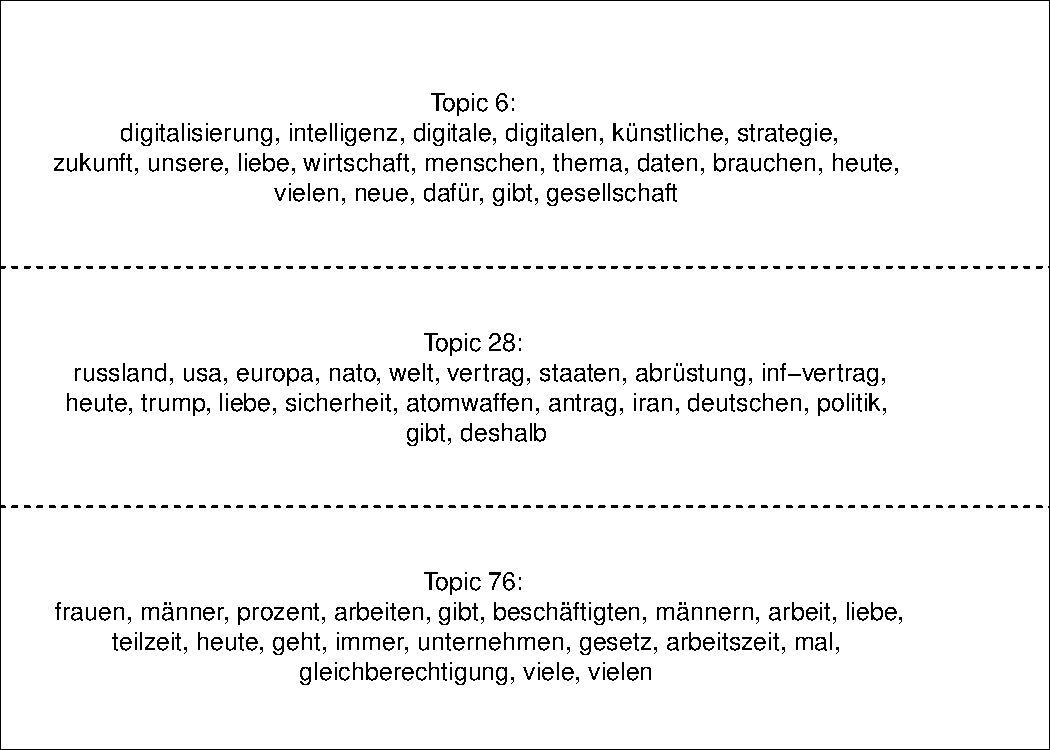
\includegraphics[width=.9\linewidth]{document/images/stm_label_prob_example.pdf}
      \caption{\emph{highest probability}}
      \label{fig:sub1}
    \end{subfigure}%
    \begin{subfigure}{.5\textwidth}
      \centering
      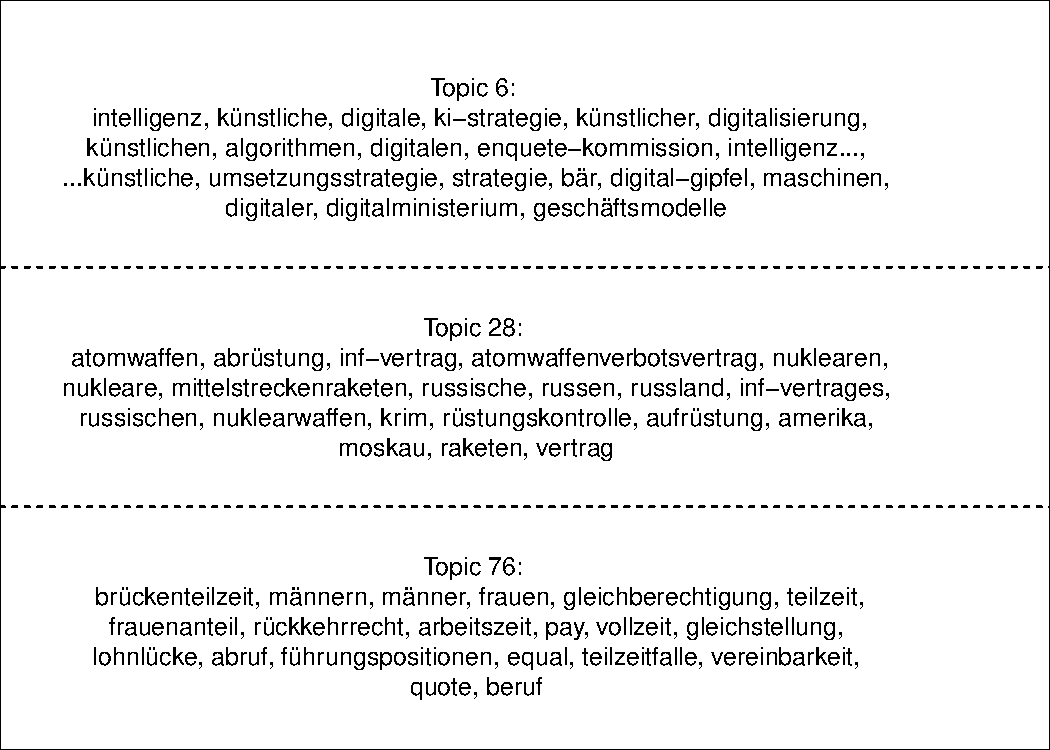
\includegraphics[width=.9\linewidth]{document/images/stm_label_frex_example.pdf}
      \caption{\emph{FREX}}
      \label{fig:sub2}
    \end{subfigure}
    \caption[Labeling am Beispiel der Topics 6, 28 und 76 mittels des \emph{highest probability} und \emph{FREX}-Algorithmus]{Labeling am Beispiel der Topics 6, 28 und 76 mittels des \emph{highest probability} und \emph{FREX}-Algorithmus.}
    \label{fig:example_labels}
\end{figure}

Das Labeling wurde unabhängig durch die beiden Autor*innen vorgenommen und anschließend die Ergebnisse verglichen. Es wurden 13 Topics aus dem Datensatz entfernt, da sie entweder aus zusammenhanglosen Wörtern oder beispielsweise nur aus Dankes- und Begrüßungswörtern bestanden. Bei 26 Topics bestand keine Einigkeit bezüglich des Labels -- hier wurden die Reden, welche am meisten den Topics zugeordnet werden können, gesichtet und anschließend das Labeling vorgenommen oder auch diese aus der Erhebung entfernt. Nach dieser Überprüfung bleiben 85 Topics, welche auf mögliche Unterschiede zwischen männlichen und weiblichen Abgeordneten untersucht werden können.

Betrachtet man die Topics, welche ein signifikantes Ergebnis bezüglich !!!Wort fehlt - der Topic-Anteile!!! zeigen (Konfidenzintervall von 80\%)

Mit Betrachtung der Topics, welche einen signifikanten Unterschied bezüglich der Topic-Anteile von männlichen und weiblichen Abgeordneten aufweisen (vgl. Abb. \ref{fig:differences_stm_top}) kann eine Reproduktion von Stereotypisierungen bezüglich der Thematisierung in den Bundestagsreden nachgewiesen werden.\footnote{Die Ergebnisse aller Topics mit dem jeweiligem Label finden sich im Anhang, vgl. Abb. \ref{fig:differences_stm}} Die Ergebnisse, welche \textcite[501ff.]{back_2014} im schwedischen Reichstag erhoben hatten, können in unserer Arbeit reproduziert werden. Auch wenn in dieser Arbeit eine Klassifizierung von \enquote{hard policies}, wie sie bei \citeauthor{back_2014} vorgenommen wurde, nicht angewandt wird, zeigt sich, dass männliche Abgeordnete signifikant mehr über Außen- und Verteidigungspolitik (INF-Vertrag, EU-Außenpolitik, Bundeswehreinsatz im Mittelmeer \enquote{Sea Guardian}) und Finanzpolitik (Steuern, Finanzen, Banken) sowie Energiepolitik im Bundestag sprechen (vgl. Abb. \ref{fig:differences_stm_top}). Diese Thematisierung entspricht in großen Teilen der Klassifizierung von \enquote{hard policies} von \citeauthor{back_2014} -- hier werden die Topics \enquote{Makroökonomie}, \enquote{Energie}, \enquote{Transportwesen}, \enquote{Bankwesen, Finanzen und Handel} sowie \enquote{Raumfahrt, Wissenschaft, Technologie und Kommunikation} als sogenannte \enquote{hard policy issues} identifiziert \parencite[510]{back_2014}. Überraschenderweise wird Außen- und Verteidigungspolitik durch \citeauthor{back_2014} nicht als \enquote{hard policy} definiert, obwohl die dieser Arbeit zugrundeliegende Untersuchung von \textcite{reynolds_1999} dieses Themenfeld als solches identifiziert \parencite[564]{reynolds_1999}.

\begin{quote}
    \enquote{The main result is that female politicians have consistently been the group that have pursued social welfare policy issues to the greatest extent in their parliamentary work.} \parencite[82]{wangnerud_2000}
\end{quote}

Allerdings finden sich in unserer Erhebung, anders als bei \textcite{back_2014}, eine signifikant mehrheitliche Thematisierung von \enquote{soft policies} \parencite[510]{back_2014} durch Frauen -- etwa zu den Themen Gesundheit (Pflege), Bildung (Studium/Bildung), und Sozialwesen (Familienpolitik). \textcite{back_2014} konnten in ihrer Untersuchung bei diesen Thematisierungen keine Unterschiede bezüglich der Häufigkeit von Reden im Bezug auf das Geschlecht feststellen \parencite[512]{back_2014}. \textcite{wangnerud_2000} fasst in ihrer Untersuchung allerdings zusammen, dass Frauen schon immer die Gruppe waren, die sich in der parlamentarischen Arbeit sozialpolitische Themen am stärksten einsetzten.

\begin{figure}[H]
    \centering
    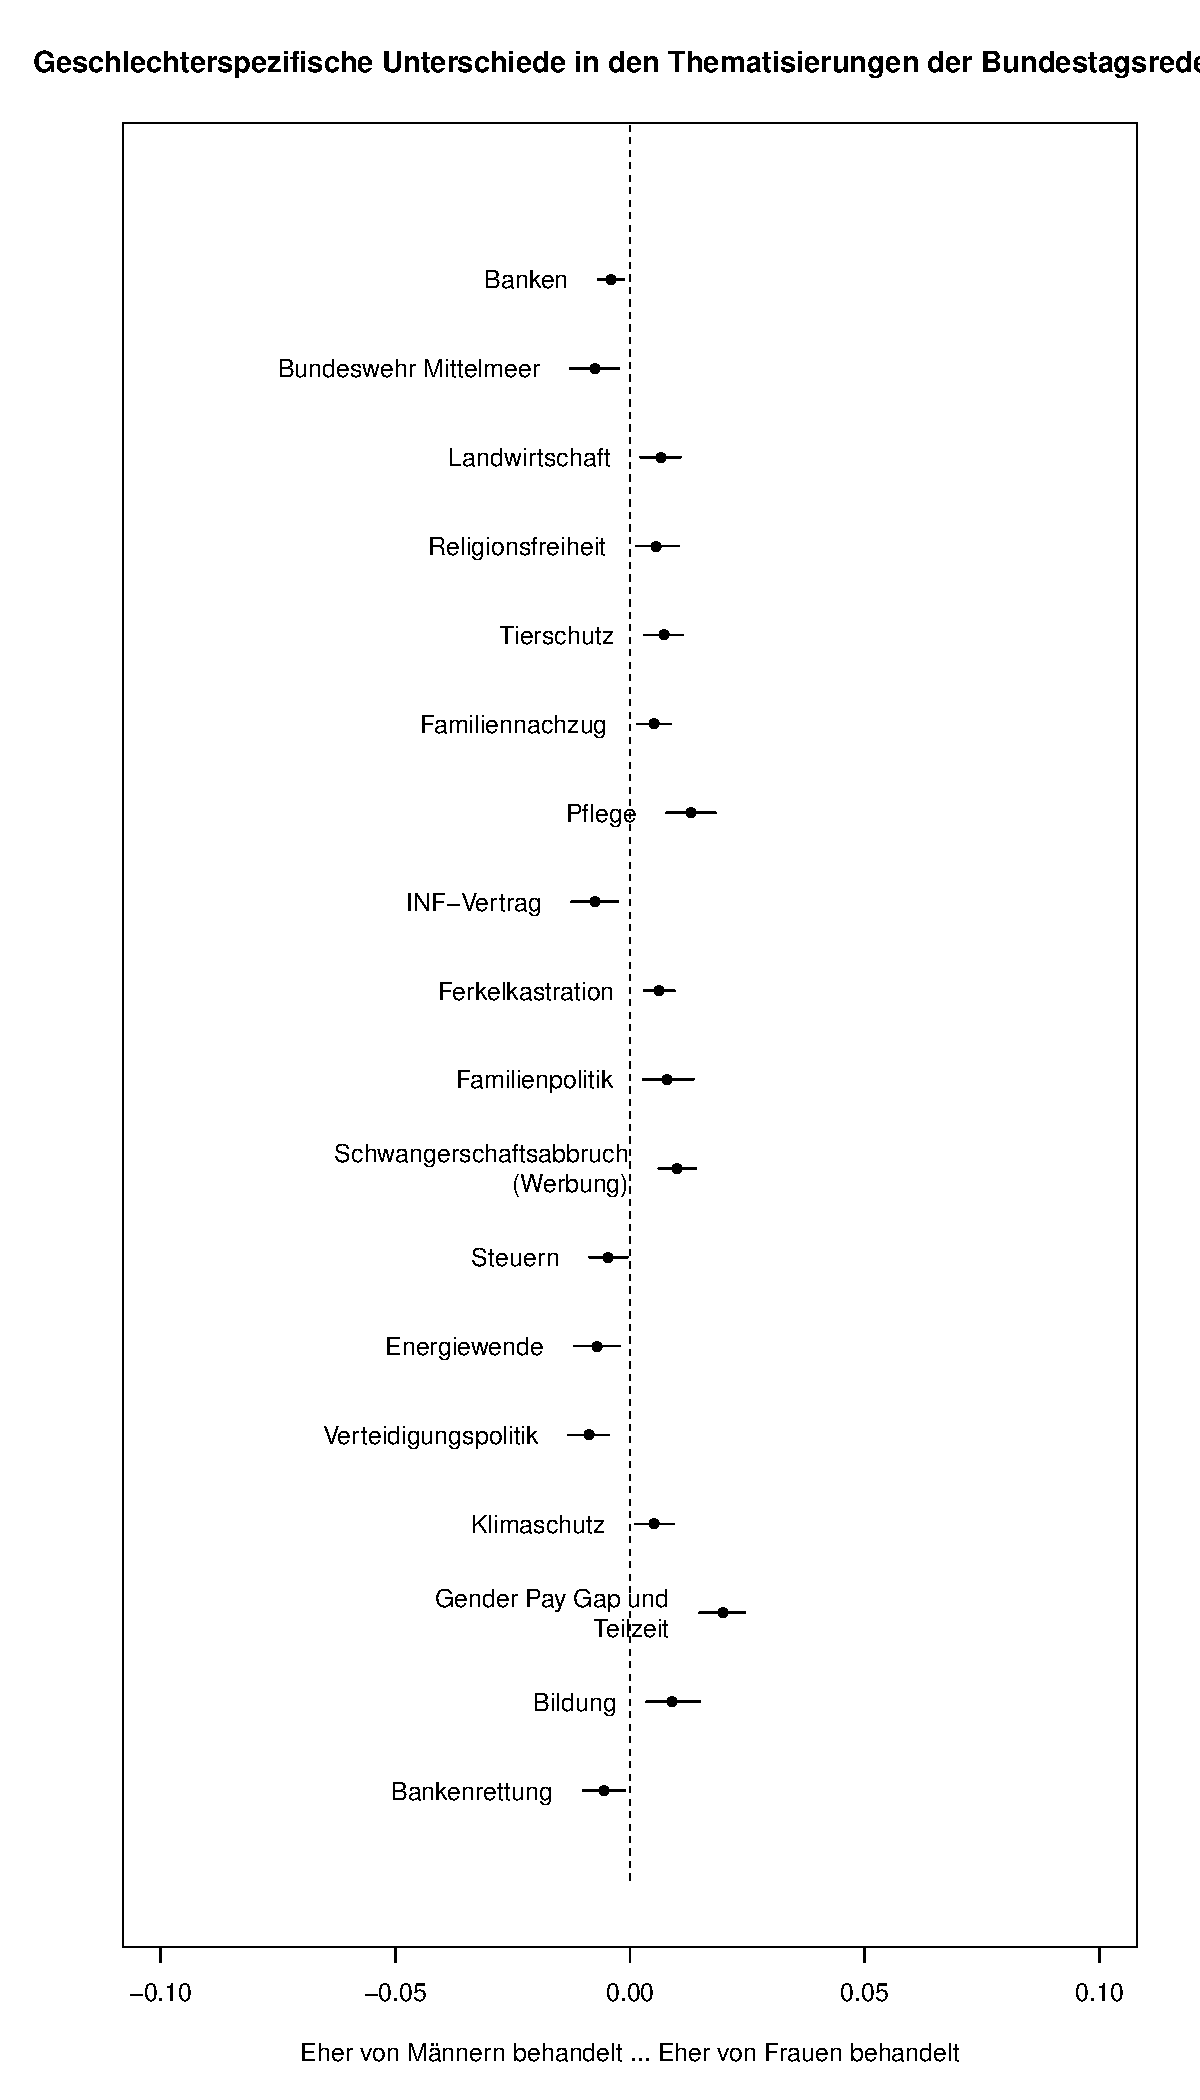
\includegraphics[scale=0.6]{images/stm_differences_top.pdf}
    \caption[Thematisierungen in den Bundestagsreden mit signifikanten Unterschieden zwischen den Geschlechtern]{Thematisierungen in den Bundestagsreden mit signifikanten Unterschieden zwischen den Geschlechtern. Diese Abbildung zeigt die Punktschätzung und das 80\% Konfidenzintervall der mittleren Differenz der Themenanteile. Tangiert das Konfidenzintervall die Nullinie, gilt das Ergebnis als nicht signifikant.}
    \label{fig:differences_stm_top}
\end{figure}

Unsere Ergebnisse zeigen, dass unterschiedliche Thematisierungen der Reden von Abgeordneten feststellbar sind -- die Nullhypothese $H_0$ (\emph{Es gibt keine Unterschiede in den Thematisierungen der Reden der Abgeordneten}) kann im Bezug auf das Geschlecht also abgelehnt werden. Es findet überwiegend eine Reproduktion von Stereotypen statt -- während Männer überwiegend zu \enquote{hard policies} sprechen, findet sich auch eine signifikanter Unterschied bei der Thematisierung von \enquote{soft policies} durch Frauen.
Da in dieser Arbeit aber keine vorherige Identifikation von \enquote{hard} und \enquote{soft policies} vorgenommen wurde und das in dieser Untersuchung gewählte Technik des \emph{structural topic modeling} auch ohne eine solche Kategorisierung möglich ist, konnten auch Topics identifiziert werden, welche keine dieser Kategorien zugeordnet werden kann. So sprechen Frauen häufiger über Klimaschutz, Landwirtschaft und Religionsfreiheit (vgl. Abb. \ref{fig:differences_stm_top}).


\begin{quote}
    There are particular needs, interests, and concerns that arise from women's experience, and these will be inadequately addressed in a politics that is dominated by men. \parencite[66]{phillips_1998}.
\end{quote}

Es zeigt sich aber auch eine Bestätigung der \emph{politics of presence} von \textcite{phillips_1998}: Die spezifischen Bedürfnisse, Interessen und Bedenken, die sich aus der Erfahrung der Frauen ergeben, werden vor allem von Frauen thematisiert -- so zum Beispiel die Themen Schwangerschaftsabbruch und Gleichberechtigung (vgl. Abb. \ref{fig:differences_stm_top}). Hierbei handelt es sich nicht um die Reproduktion von Stereotypen, sondern die spezifische Wahrnehmung von Themen, welche explizit Frauen betreffen.


\section{Unterbrechungen}

\todo[inline]{Ein großer Teil der Reden kommt ohne negative Unterbrechungen (Lachen, Zuruf, Gegenruf, Widerspruch) aus (vgl. Abb. \ref{fig:histo_reden_unterbrechung}}

\begin{figure}
    \centering
    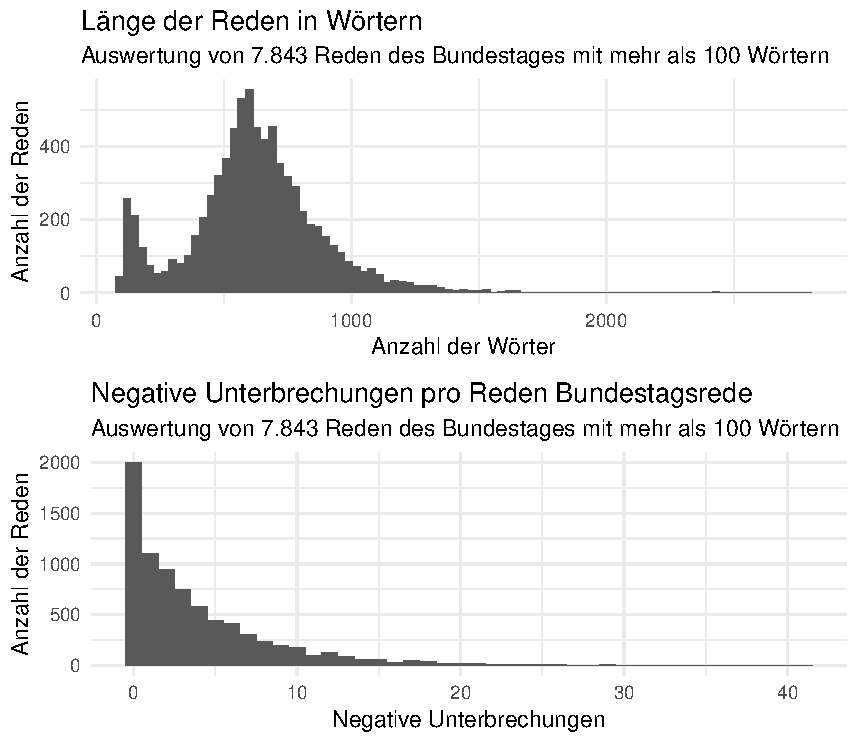
\includegraphics{images/histogram_unterbrechung.pdf}
    \caption{Histogramme zu Anzahl der Wörter und Anzahl an Unterbrechungen der Reden im 19. Deutschen Bundestage}
    \label{fig:histo_reden_unterbrechung}
\end{figure}

\Chapter{Methodenkriktik und Forschungsausblick}

\todo[inline]{Stichpunkte: 

GFL: 


PROBLEM: 
Das Genderdiktionär ist  ungenügend für die vorliegende Forschungsarbeit und bedarf weiterer interdisziplinärer Ausarbeitung. Die Begriffe sind teilweise zu unspezifisch (BEISPIELE?) oder \emph{zu} spezifisch (BEISPIEL?). Aufgrund des fehlenden Domänenbezuges ist es problematisch die Wörter des Diktionärs ohne weitere Prüfung zu nutzen (BEISPIELE?). 

LÖSUNG: 
Das hier verwendete Gender-Diktionär wurde von Laien ausgearbeitet und hat eine Vielzahl an Schwachstellen. Mit Blick auf die Zukunft ist es notwendig ein Gender-Diktionär interdisziplinär mit LInguist*innen und Wissenschaftlier*innen des jeweilgen Fachbereichs bzw. der jeweiligen Domäne auszuarbeiten
????!!!!! (crowd - JH?) und hasselmeier und jenny: wörterbücher immer hohe domänenabhängigkeit, daher spezifisch Politik-wörterbuch notwendig !!!!!

Problem: In den Protokollen des Deutschen Bundestags sind keine \emph{Gender Gaps} verzeichnet. AUfgrund dessen werden diese in den Protokollen als weibliche Form abgespeichert (bspw. Student\_innen \= Studentinnen), wodurch die Ermittlung von GFL (in der Form \emph{Gender Gaps}) mit den hier verwendeten Methoden unmöglich ist.

Lösung: Um dieses Problem zukünftig zu vermeiden, wären Audiodateien -- aus denen die gesprochene Lücke hervorgeht -- notwendig. Alternativ könnten die \emph{Gender Gaps} in den Protokollen verzeichnet werden um eine spätere Auswertung zu ermöglichen. 

Problem: Die 10 meistverwendeten GFL-Formulierungen schließen auf Platz 1 \emph{Kolleginnen und Kollegen} sowie u.a. \emph{Damen und Herren}, \emph{Bürgerinnen und Bürger} mit ein. Problematisch ist hierbei, dass diese Formulierungen in nahezu jeder Ansprache vorkommen (SIEHE WO?) und die vorliegenden Daten hinsichtlich der Nutzung von GFL-Formulierungen verzerren. 

Lösung: 
Diese Feststellung lässt zusammen mit den Problematiken des GEdner-Diktionärs darauf schließen, dass die vorliegende Auswertung zur Nutzung von GFL nicht auszuwerten ist. Wenngleich eine hohe Signifikanz in dem hier verwendeten Modell festgestellt werden konnte, ist die methodologische Konzeption zu fehleranfällig um die vorliegenden Ergebnisse zu veröffentlichen. 
Die weitere Konzeption, Ausarbeitung und Bereitstellung einer domänenbezogenen Diktionärs (inklusive \emph{GFL-Begriffe} und \emph{GFL-Formulierungen}) für zukünftige Forschung ist unumgänglich um eine zukünftige Analyse der notwendigen Verwendung von GFL zu ermöglichen und zu fördern.

THEMEN: 

THEMEN: 


bäck sagte automatic analyse könnte genutzt werden, dies haben wir gemacht - was einerseits die ergebnisse vn wängerud bestätigt - welche sie hart und soft nannte - wir kommen auf ähnlich themen - ohne vorherige einteilung in hard und soft, auch themen identifizierbar welche vorher nicht einzuordnen waren/ entdeckt worden wären
Ohne eine vorherige Einteilung des Themen in \emph{soft} und \emph{hard policies} konnten wir ähnliche Ergebnisse (???können wir das so schreiben!!!!) im Deutschen Bundestag erzielen wie \textcites[505]{back_2014} im Schwedischen \emph{Riksdag}\parencite[vgl. auch][]{wangnerud_1996}. 





Problem:
bäck 2018 - 'brauchen einen besseren zugang zu daten' - (zur Lösung:)wir haben unsere bisherige forschung frei zugänglich gemacht um weitere arbeit mit unseren daten zu ermöglichen... 

LÖSUNG:
Daten zugänglich machen 
unsere daten können als ausgangspunkt verwendet werden ... 



UNTERBRECHUNGEN:

PROBLEM

LÖSUNG 

Problem

Eine weitere zu Untersuchende Hypothese könnte lauten: {Frauen erfahren häufiger Rückfragen in ihren Reden, wenn wenige andere Frauen zu diesem Thema gesprochen haben}.\footnote{Diese Hypothese kann nur in Verbindung mit der Hypothese 3 zur Thematisierung in den Reden überprüft werden.} Dieser Hypothese würde die Annahme zugrunde liegen, dass Frauen eher durch Rückfragen unterbrochen werden, da Ihnen in diesen Themen Inkompetenz unterstellt wird. Die vorliegende Arbeit hat mit Hinblick auf die Topics einen ersten Teil der Analyse gestellt und weitergehende Forschung ist wünschenswert.


ANALYSE DES ARBEITSPLATZES; 

 Unterbrechungen im plenum haben wir untersucht  

weiter forschung ist notwendig um den arbeitsplatz zu analysieren -... z.b in form von Befragungen der MPs  - um zu untersuchen ob es sich um eine gendered instistution / maskuline Orga handelt??? 

1. mal rechtspop partei im bundestag - viele unterbrechungen bzgl. AFD ...provozieren mit Reden (Josef anhang) - spannend zu untersuchen wie sich das verhalten der abgeorndeten (AUCH in bezug auf geschlechterbezogenes VErhalten) verändert hat

auch die Frage : WER unterbricht? das war nicht gegenstand dieser Arbeit - weiter Forschung wünschenwert 

EBENEN AUSWERTEN!!!!!
}

\Chapter{Fazit}\label{kapitel:diskussion}

!!!!Einleitung für das folgende ZITAT!!!WOHIN DIE FOLGENDEN ZITATE????!!!

%

\begin{quote}
    \enquote{Although women remain significantly under-represented in today’s parliaments, they are now looking beyond the numbers to focus on what they can actually do while in parliament — how they can make an impact, whatever their numbers may be. They are learning the rules of the game and using this knowledge and understanding to promote women’s issues and concerns from inside the world’s legislatures. In so doing, they are not only increasing the chances of their own success, but they are also paving the way for a new generation of women to enter the legislative process.} \parencite[3]{lovenduski_2015}
\end{quote}
%
\citereset
\begin{quote}
    \enquote{Gender equal representation is not only about the proportion of men and women legislators or the outcomes of politics}\parencite[197]{erikson_2018}
\end{quote}

(!!!WOHIN die obigen Zitate?)

Zur Analyse von geschlechtsbezogenen Repräsentationsunterschieden im Deutschen Bundestag werden zunächst fünf Repräsentations-Dimensionen definiert und differenziert voneinander betrachtet. 
\begin{itemize}
    \item Ebene A: \emph{Repräsentation von Frauen im Parlament}: Sind Frauen im Parlament vertreten? Wie viele Frauen sind relativ und absolut im Parlament vertreten? 
    \item Ebene B: \emph{Beteiligung von weiblichen MPs an den Parlamentsdebatten}: Nehmen weibliche MPs absolut und relativ (in Bezug auf die Anzahl an Sitzen im Parlament) gleich viel an den Parlamentsdebatten teil wie männliche MPs? 
    \item Ebene C: \emph{Berücksichtigung von Frauen in der Sprache der Parlamentsdebatten}: Werden in den Debatten Frauen ebenso wie Männer sprachlich repräsentiert? Wird Gender-Fair-Language (GFL) genutzt? Wird GFL von weiblichen und männlichen MPs in gleichem Maße genutzt? 
    \item Ebene D: \emph{Vermeidung von geschlechtsbezogenen Stereotypisierungen}: Werden gesellschaftliche geschlechtsbezogene Stereotypisierungen reproduziert? Werden unterschiedliche Themen von weiblichen und männlichen MPs behandelt? Gibt es thematische Unterschiede innerhalb der Reden zu den gleichen Themen zwischen männlichen und weiblichen MPs? 
    \item Ebene E: \emph{Verhinderung von frauenfeindlichen Verhaltensmustern}: Werden in den Parlamentsdebatten frauenfeindliche Verhaltensmuster reproduziert? Werden Frauen häufiger negativ unterbrochen? 
    \end{itemize}

(ALS FUßNOTE:)Wenngleich keine dieser Dimension gänzlich unabhängig von den anderen Dimensionen analysiert werden kann, werden sie in dieser Arbeit zunächst klar voneinander getrennt um die Komplexität der verschiedenen Dimensionen zu reduzieren. Nicht alle 5 Ebenen konnten jedoch mit einem \emph{Repräsentationsbegriff} erfasst werden. Dies scheitert an Ebene D und E --bei diesen Ebenen handelt es sich um eine Reproduktion - sihee Kapitel xy). 


\todo[inline]{Mit Blick auf die unterschiedlichen Ebenen  ---- Repräsentationsbegriff --- Überleitung ??!??!?!?!}

Die Theorie des \emph{Workplace-Approach} von \textcite{erikson_2018} und das Konzept der \enquote{\emph{culture of masculinity}} von \textcite{lovenduski_2005} sowie \textcite{erikson_2018} dargestellt bilden den Ausgangspunkt dieser Arbeit. Eine geschlechtergerechte Repräsentation wird in dieser Arbeit weder ausschließlich daran gemessen, ob eine gleiche Anzahl an Frauen und Männern im Parlament vertreten ist (A), noch anhand der politischen Ergebnisse. Ein Ausgangspunkt der vorliegenden Arbeit ist, dass das legislative Arbeitsumfeld für sich genommen ebenso wichtig ist \emph{\enquote{workplace approach}}, wie die Möglichkeiten der weiblichen Gesetzgeberinnen die Ergebnisse zu beeinflussen. Sowohl Beteiligung von weiblichen MPs an den Parlamentsdebatten (B), die Berücksichtigung von Frauen in der Sprache der Parlamentsdebatten (C) die Vermeidung von geschlechtsbezogenen Stereotypisierungen (D) als auch die Verhinderung von frauenfeindlichen Verhaltensmustern (E) fallen unter das legislative Arbeitsumfeld. 
Innerhalb des Arbeitsumfeldes können informelle Praktiken und Normen als Hindernis für die Schaffung eines geschlechtergerechten Arbeitsumfeldes fungieren \parencite[200]{erikson_2018}. Es wird vermutet, dass informelle Aspekte des Arbeitsumfelds im Parlament in einer Weise geschlechtsspezifisch sind, dass weibliche MPs trotz ihrer formalen und deskriptiven Geschlechtergleichstellung benachteiligt werden \parencite[210]{erikson_2018}. Ausgangspunkt der vorliegenden Arbeit ist die Annahme, dass der 19. Deutschen Bundestag ebenfalls von einer \enquote{\emph{culture of masculinity}} geprägt ist und dies neben weiteren Faktoren die Geschlechtergerechtigkeit des Arbeitsumfeldes zum Nachteil von Frauen beeinflusst.
Wenngleich die Relevanz von Geschlechtergleichheit auf politischer Ebene nicht in Frage gestellt werden kann gibt es Uneinigkeit darüber, ob -- und auf welchen Ebenen -- eine  Gleichstellung der Geschlechter bereits abgeschlossen oder nahezu umgesetzt wurde.

Die Forderungen einer deskriptiven parlamentarischen Geschlechtergleichheit haben ebenso wie die Forderungen nach substantieller Geschlechtergleichheit bereits ihre Wege in die wissenschaftliche Diskussion und in die Politik gefunden. Einer geschlechtergerechten Sprache sowie dem geschlechtsbezogenen Verhalten im Parlament wurde bisher allerdings weniger Aufmerksamkeit gewidmet, obwohl \emph{Sprache} in Anlehnung an \textcite{menegatti_2017} eine der einflussreichsten Faktoren darstellt, wodurch Sexismus und Geschlechterdiskriminierung gefördert und reproduziert werden \parencite*[1]{menegatti_2017}.

Um geschlechtsbezogene Repräsenatationsunterschiede auf allen fünf Ebenen zu analysieren wird die Frage ‚Inwiefern unterscheiden sich Redebeiträge und Verhalten von weiblichen und männlichen Abgeordneten im 19. Deutschen Bundestag bezüglich Häufigkeit, Thematik und Geschlechterneutralität?‘ wird mit Hilfe von drei übergeordneten Hypothesen untersucht:
\begin{itemize}
    \item H1 : Weibliche MPs verwenden in ihren Reden häufiger GFL als männliche MPs
    \item H2: Es sind unterschiedliche Thematisierungen in den Reden der Abgeordneten feststellbar
    \item H3: Frauen werden häufiger als Männer während einer Rede negativ Unterbrochen)
\end{itemize}



!!!Die Ergebnisse: ... 





\begin{appendices}
\chapter{Anhang}

\begin{figure}[H]
    \centering
    \includegraphics[page=14,scale=0.7]{images/protokoll_beispiel.pdf}
    \caption{Auszug des Plenarprotokolls 19/96 von 12.04.2016}
    \label{fig:protokoll_bsp}
\end{figure}


\begin{figure}
  \centering
   \begin{tabular}{@{}c@{\hspace{.5cm}}c@{}}
       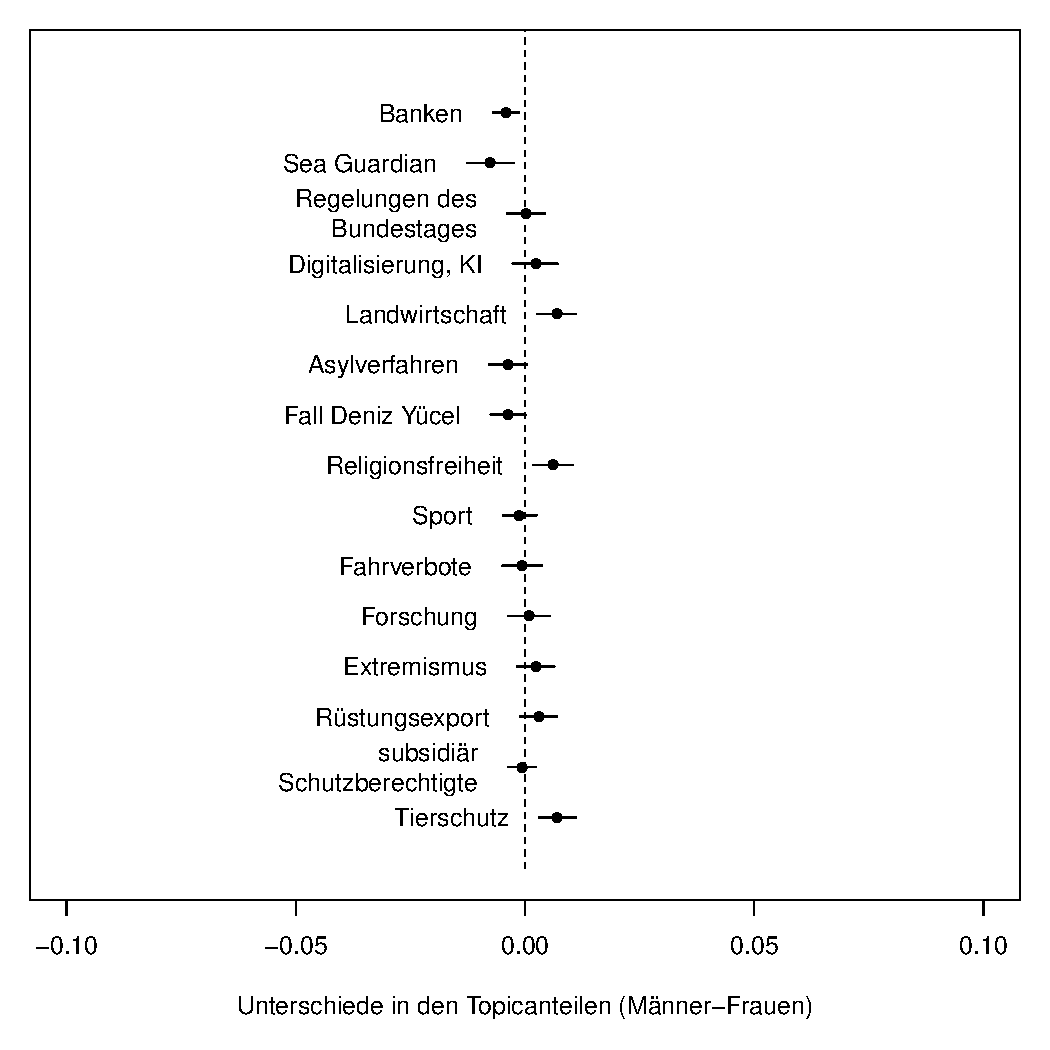
\includegraphics[page=1,width=.45\textwidth]{images/stm_differences.pdf} & 
       \includegraphics[page=2,width=.45\textwidth]{images/stm_differences.pdf} \\
       \includegraphics[page=3,width=.45\textwidth]{images/stm_differences.pdf} &
       \includegraphics[page=4,width=.45\textwidth]{images/stm_differences.pdf} \\
       \includegraphics[page=5,width=.45\textwidth]{images/stm_differences.pdf} &
       \includegraphics[page=6,width=.45\textwidth]{images/stm_differences.pdf}
   \end{tabular}
    \caption[Thematisierungen in den Bundestagsreden nach Geschlecht der Abgeordneten]{Thematisierungen in den Bundestagsreden (!!!!Parlamentsdebatten?!!!ÜBERALL EINHEITLICH !!!!! ODER ?!!!!!!) nach Geschlecht der Abgeordneten. Diese Abbildung zeigt die Punktschätzung und das 80\% Konfidenzintervall der mittleren Differenz der Themenanteile. Tangiert das Konfidenzintervall die Nullinie, gilt das Ergebnis als nicht signifikant.}
    \label{fig:differences_stm}
\end{figure}
\end{appendices}



\section{Kontrollvariablen}

Die Anzahl an Unterbrechungen und die Nutzung genderinklusiver Sprache wird von mehr Faktoren als nur dem Geschlecht beeinflusst -- linke Parteien nutzen vermutlich häufiger genderinklusive Sprache als rechte Parteien, Fraktionsvorsitzende werden vermutlich häufiger unterbrochen als MPs, welche nicht den (stellvertretenden) Fraktionsvorsitz stellen.
Anbei sollen einige Kontrollvariablen aufgeführt werden, welche bei den Hypothesen ebenfalls geprüft werden. Da es sich bei dieser Arbeit um eine x-zentrierte Forschungsfrage handelt (\emph{Inwiefern unterscheiden sich Redebeiträge und Verhalten von weiblichen und männlichen Abgeordneten im 19. Deutschen Bundestag bezüglich Häufigkeit, Thematik und Geschlechterneutralität}) \parencite[vgl.][4f.]{ganghof_2005} wird untersucht, inwiefern das Geschlecht eine Rolle bei den untersuchten Hypothesen spielt: 


\begin{itemize}
    \item Geschlecht ist nur eine von vielen Variablen, welche sich beispielsweise auf die Anzahl der Unterbrechungen in einer Bundestagsrede auswirken könnte. Es ist davon auszugehen, dass Fraktionsvorsitzende z. B. während ihrer Reden häufiger unterbrochen werden als Abgeordnete, welche nicht den Vorsitz stellen.
    \item Es handelt sich bei dieser Arbeit um eine x-zentrierte Forschungsfrage \parencite[vgl.][4f.]{ganghof_2005}- inwiefern spielt das Geschlecht eine Rolle?
    \item Mit Kontrollvariablen kann das Risiko einer Scheinkorrelation minimiert werden, da auf mehr Faktoren als nur das geschlecht kontrolliert wird
    \item Neben den Variablen, bei denen ein Einfluss auf die zu überprüfenden abhängigen Variablen erwartet wird (beispielsweise Fraktionsvorsitz, Mitglied der Opposition) sollen auch Variablen, überprüft werden, bei denen keine Auswirkungen auf den Untersuchungsgegenstand erwartet wird -- beispielsweise das Alter des*der Redner*in bezüglich der Anzahl der Unterbrechungen.
    \item Wie die Fragestellung \enquote{Inwieweit unterscheiden sich die Redebeiträge und Verhalten von weiblichen und männlichen Abgeordneten im 19. Deutschen Bundestag bezüglich Häufigkeit, Thematik und Geschlechterneutralität} bereits suggeriert, wird davon ausgegangen, dass die Variable \emph{Geschlecht} einer von vielen Faktoren ist, welche das Verhalten, die Sprache und den Inhalt der Bundestagsdebatte beeinflussen. Entsprechend handelt es sich bei dieser Untersuchung um ein x-zentriertes Forschungsdesign, in welchem auch weitere Faktoren, welche auf die jeweilige abhängige Variable einwirken, untersucht werden sollen  \parencites[vgl.][3f.]{ganghof_2005}.
    \item Überprüft werden mit diesen Kontrollvariablen die Unterbrechungen und Rückfragen. 
\end{itemize}




\setstretch{1.0}
\backmatter
\printbibliography[title={Literaturverzeichnis}]

\end{document}

\end{document}